\documentclass{rapportENSIAS}
% rapportENSIAS.cls charge déjà :
%   babel[french], inputenc[utf8], fontenc[T1], graphicx, subcaption,
%   hyperref[hidelinks], geometry, fancyhdr, mathtools, float, titlesec, tocloft

% ============================================================
%  PACKAGES SUPPLÉMENTAIRES (non inclus dans la classe)
% ============================================================
\usepackage{lmodern}
\usepackage{microtype}

% Math
\usepackage{amsmath,amssymb}

% Tables
\usepackage{booktabs}
\usepackage{multirow}
\usepackage{array}
\usepackage{longtable}
\usepackage{tabularx}

% Figures / TikZ
\usepackage{tikz}
\usepackage{pgfplots}
\usepackage{pgfplotstable}
\pgfplotsset{compat=1.18}
\usetikzlibrary{arrows.meta, positioning, shapes.geometric, shapes.misc,
                fit, backgrounds, calc, decorations.pathreplacing,
                patterns, shadows, matrix, chains, scopes}

% Couleurs
\usepackage{xcolor}

% Boîtes tcolorbox
\usepackage{tcolorbox}
\tcbuselibrary{skins, breakable, listings, theorems}

% Code source (annexes uniquement)
\usepackage{listings}

% Typographie / citations
\usepackage{csquotes}
\usepackage{setspace}

% Bibliographie — natbib avec style numérique
\usepackage[numbers,sort&compress]{natbib}

% IfFileExists already available in latex kernel

% ============================================================
%  COULEURS
% ============================================================
\definecolor{primary}{RGB}{0,84,166}
\definecolor{secondary}{RGB}{0,150,214}
\definecolor{accent}{RGB}{255,140,0}
\definecolor{success}{RGB}{34,139,34}
\definecolor{danger}{RGB}{220,50,47}
\definecolor{lightblue}{RGB}{230,242,255}
\definecolor{lightyellow}{RGB}{255,253,230}
\definecolor{lightgreen}{RGB}{230,255,237}
\definecolor{codebg}{RGB}{248,248,248}
\definecolor{gray80}{RGB}{80,80,80}
\definecolor{gray50}{RGB}{127,127,127}

% ============================================================
%  BOÎTES TCOLORBOX
% ============================================================
\newtcolorbox{infobox}[1][]{%
  colback=lightblue, colframe=primary,
  fonttitle=\bfseries, title=#1, breakable,
  enhanced, shadow={0.5mm}{-0.5mm}{0mm}{gray!30}}

\newtcolorbox{resultatbox}[1][]{%
  colback=lightgreen, colframe=success,
  fonttitle=\bfseries, title=#1, breakable,
  enhanced, shadow={0.5mm}{-0.5mm}{0mm}{gray!30}}

\newtcolorbox{alertbox}[1][]{%
  colback=lightyellow, colframe=accent,
  fonttitle=\bfseries, title=#1, breakable,
  enhanced, shadow={0.5mm}{-0.5mm}{0mm}{gray!30}}

\newtcolorbox{criticalbox}[1][]{%
  colback=danger!10, colframe=danger,
  fonttitle=\bfseries, title=#1, breakable,
  enhanced, shadow={0.5mm}{-0.5mm}{0mm}{gray!30}}

% ============================================================
%  STYLE LISTINGS (pour les annexes uniquement)
% ============================================================
\lstdefinestyle{pythonstyle}{
  backgroundcolor=\color{codebg},
  commentstyle=\color{gray50}\itshape,
  keywordstyle=\color{primary}\bfseries,
  stringstyle=\color{success},
  numberstyle=\tiny\color{gray50},
  basicstyle=\ttfamily\small,
  breakatwhitespace=false,
  breaklines=true,
  captionpos=b,
  keepspaces=true,
  numbers=left,
  numbersep=6pt,
  showspaces=false,
  showstringspaces=false,
  showtabs=false,
  tabsize=4,
  frame=single,
  framerule=0.5pt,
  rulecolor=\color{gray50},
  xleftmargin=15pt
}
\lstset{style=pythonstyle, language=Python}

% ============================================================
%  INFORMATIONS DU RAPPORT
% ============================================================
\titre{Plateforme MLOps pour la Détection Précoce\\
       du Risque d'Hospitalisation}
\UE{Spécialité : Machine Learning Operations (MLOps)}
\sujet{Projet de Fin d'Années --- Santé / IA Médicale}
\enseignant{[NOM ENCADRANT]}
\eleves{Mohamed \textsc{Ettaouil}}
\jury{[NOM JURY 1] \\ [NOM JURY 2]}

% ============================================================
%  DOCUMENT
% ============================================================
\begin{document}

\fairemarges
\fairepagedegarde

% -------- Pages liminaires --------
\chapter*{Remerciements}
\addcontentsline{toc}{chapter}{Remerciements}
\input{Chapters/remerciement}

\chapter*{Résumé}
\addcontentsline{toc}{chapter}{Résumé}
Ce projet présente le développement d'une plateforme MLOps complète pour la
détection précoce du risque d'hospitalisation chez les patients polypathologiques.
À partir du dataset CMS~DE-SynPUF (30\,000 patients, données 2008--2010), trois
modèles ont été entraînés avec un split temporel strict : Régression Logistique
(AUC~0.908), XGBoost (AUC~0.924) et LightGBM (AUC~0.921). Le modèle XGBoost
retenu est déployé via une API FastAPI, conteneurisé avec Docker et supervisé par
un pipeline de monitoring Evidently/Grafana avec rollback automatique.
L'analyse de fairness démontre un écart maximal de 5.5\,\% en rappel entre groupes
raciaux. Le ROI estimé est de \$2.59~M sur la cohorte de 30\,000 patients.

\vspace{1em}
\noindent\textbf{Mots-clés :} MLOps, détection risque hospitalisation, XGBoost,
FastAPI, Docker, monitoring, data drift, fairness, CMS DE-SynPUF.

\chapter*{Abstract}
\addcontentsline{toc}{chapter}{Abstract}
This project presents a complete MLOps platform for early detection of
hospitalization risk among multi-morbid patients. Using the CMS~DE-SynPUF
dataset (30,000 patients, 2008--2010), three models were trained with strict
temporal splitting: Logistic Regression (AUC~0.908), XGBoost (AUC~0.924) and
LightGBM (AUC~0.921). The selected XGBoost model is deployed via a FastAPI,
containerized with Docker and monitored by an Evidently/Grafana pipeline with
automatic rollback. Fairness analysis shows a maximum recall gap of 5.5\%
across racial groups. Estimated ROI is \$2.59M on the 30,000-patient cohort.

\vspace{1em}
\noindent\textbf{Keywords:} MLOps, hospitalization risk detection, XGBoost,
FastAPI, Docker, monitoring, data drift, fairness, CMS DE-SynPUF.

\chapter*{Liste des Abréviations}
\addcontentsline{toc}{chapter}{Liste des Abréviations}
\begin{tabular}{@{}lp{10cm}@{}}
\toprule
\textbf{Sigle} & \textbf{Définition} \\
\midrule
AUC  & Area Under the Curve (Aire sous la courbe ROC) \\
BPCO & Bronchopneumopathie chronique obstructive \\
CI/CD & Continuous Integration / Continuous Deployment \\
CMS  & Centers for Medicare \& Medicaid Services \\
DVC  & Data Version Control \\
EDA  & Exploratory Data Analysis (Analyse exploratoire) \\
GE   & Great Expectations \\
MLOps & Machine Learning Operations \\
PSI  & Population Stability Index \\
ROC  & Receiver Operating Characteristic \\
ROI  & Return on Investment \\
SHAP & SHapley Additive exPlanations \\
VP   & Vrai Positif \\
FP   & Faux Positif \\
VN   & Vrai Négatif \\
FN   & Faux Négatif \\
\bottomrule
\end{tabular}

\tabledematieres

\listoffigures
\addcontentsline{toc}{chapter}{Table des figures}

\listoftables
\addcontentsline{toc}{chapter}{Liste des tableaux}

% -------- Corps --------
\chapter*{Introduction Générale}
\addcontentsline{toc}{chapter}{Introduction Générale}
\markboth{Introduction Générale}{Introduction Générale}

\begin{infobox}[Contexte général]
Les systèmes de santé font face à une pression croissante~: vieillissement de la
population, multiplication des maladies chroniques et explosion des coûts
hospitaliers. Selon l'OCDE, les hospitalisations évitables représentent jusqu'à
\textbf{15\,\% des dépenses hospitalières} dans les pays développés, soit plusieurs
milliards de dollars chaque année.
\end{infobox}

\vspace{1em}

\noindent L'émergence du \textbf{Machine Learning Operations (MLOps)} offre une
réponse concrète à ce défi~: industrialiser les modèles d'intelligence artificielle
pour qu'ils produisent une valeur réelle, continue et fiable en production, et non
uniquement dans des notebooks de recherche. Ce projet se situe précisément à
l'intersection de la santé numérique et du MLOps.

\section*{Contexte et problématique}

Le dataset CMS~DE-SynPUF (Centers for Medicare \& Medicaid Services) constitue
l'une des bases de données médicales synthétiques les plus complètes et réalistes
disponibles publiquement. Il couvre 2,3~millions de bénéficiaires sur la période
2008--2010, avec plus de 60~Go de données incluant les claims d'hospitalisation,
de consultations ambulatoires, de prescriptions et de données démographiques.

\noindent La problématique centrale de ce projet est la suivante~:

\begin{criticalbox}[Question de recherche]
\textit{Comment construire un système de prédiction du risque d'hospitalisation
suffisamment fiable pour guider des interventions préventives, tout en garantissant
que ce système reste opérationnel, équitable et traçable au fil du temps~?}
\end{criticalbox}

\noindent Cette question soulève plusieurs défis~:
\begin{itemize}
  \item le \textbf{déséquilibre de classes} (seuls 8.1\,\% des patients sont
        hospitalisés dans l'année) ;
  \item la \textbf{fuite de données temporelle} (\textit{data leakage}) si la
        variable cible est mal construite ;
  \item la \textbf{dérive des données} dans le temps, qui dégrade les performances
        sans qu'on s'en rende compte ;
  \item les \textbf{biais algorithmiques} qui pénalisent certains groupes raciaux
        et socio-économiques.
\end{itemize}

\section*{Objectifs du projet}

Ce projet vise à concevoir, entraîner, déployer et surveiller une plateforme MLOps
complète pour la détection précoce du risque d'hospitalisation. Les objectifs
spécifiques sont~:

\begin{enumerate}
  \item Réaliser une \textbf{analyse exploratoire} rigoureuse et une ingénierie
        des données anti-leakage sur le dataset CMS~DE-SynPUF.
  \item Entraîner et optimiser \textbf{trois modèles} (Régression Logistique,
        XGBoost, LightGBM) avec un split temporel strict et une optimisation
        d'hyperparamètres par Optuna.
  \item \textbf{Déployer} le meilleur modèle via une API FastAPI conteneurisée
        avec Docker.
  \item Mettre en place un \textbf{pipeline de monitoring} automatique (Evidently,
        Grafana) avec détection de dérive et rollback.
  \item Évaluer l'\textbf{équité algorithmique} par groupe racial et calculer le
        ROI financier de la solution.
\end{enumerate}

\section*{Plan du rapport}

Ce rapport est organisé en quatre chapitres~:

\begin{itemize}
  \item \textbf{Chapitre~1 — Comprendre le Problème avant de le Résoudre~:}
        définition du MLOps, contexte médical, description du dataset, stack
        technologique et architecture globale du système.

  \item \textbf{Chapitre~2 — De la Donnée Brute à la Donnée Prête~:}
        analyse exploratoire complète, nettoyage des données, construction
        anti-leakage de la variable cible, fenêtres temporelles et ingénierie
        des 29 features finales.

  \item \textbf{Chapitre~3 — Apprendre à Prédire : Modèles et Expérimentation~:}
        traitement du déséquilibre, entraînement et comparaison des modèles,
        optimisation du seuil de décision, interprétabilité SHAP, traçabilité
        MLflow et analyse ROI.

  \item \textbf{Chapitre~4 — Du Modèle au Service : Mise en Production~:}
        API FastAPI, conteneurisation Docker, CI/CD GitHub~Actions, monitoring
        de la dérive, rollback automatique, analyse de fairness et bilan des
        tests réalisés.
\end{itemize}

% ============================================================
%  CHAPITRE 1 : Comprendre le Problème avant de le Résoudre
% ============================================================
\chapter{Comprendre le Problème avant de le Résoudre}
\label{chap:contexte}

\begin{infobox}[Résumé du chapitre]
Ce chapitre pose les fondations du projet~: définir ce qu'est le MLOps et
pourquoi il est indispensable en santé, caractériser la problématique médicale,
décrire le dataset CMS~DE-SynPUF, présenter la stack technologique retenue et
illustrer l'architecture globale du pipeline.
\end{infobox}

% ============================================================
\section{Le MLOps~: industrialiser l'IA pour qu'elle tienne ses promesses}
% ============================================================

\subsection{De la recherche à la production~: un fossé difficile à franchir}

Les prévisions de la littérature académique et des rapports industriels
convergent~: \textbf{plus de 85\,\% des projets de machine learning ne parviennent
jamais en production}~\cite{sculley2015hidden, zaharia2018accelerating}. Cette
statistique, souvent citée, recouvre une réalité concrète~: un modèle entraîné
dans un notebook peut obtenir d'excellentes métriques en validation, et pourtant
échouer à produire de la valeur lorsqu'il est confronté aux flux de données réels,
aux contraintes d'infrastructure ou à l'évolution du comportement des données dans
le temps.

Le terme \textbf{MLOps} --- contraction de \textit{Machine Learning} et
\textit{Operations} --- désigne l'ensemble des pratiques, outils et processus visant
à réduire ce fossé. Il s'inspire du mouvement DevOps qui a transformé le
développement logiciel, en y ajoutant les contraintes spécifiques aux systèmes
d'apprentissage automatique~: gestion des données, versionnement des modèles,
reproductibilité des expériences et surveillance de la dérive.

\subsection{Les huit principes du MLOps}

\begin{table}[htbp]
\centering
\caption{Les huit principes fondamentaux du MLOps}
\label{tab:principes_mlops}
\begin{tabularx}{\textwidth}{@{}lX@{}}
\toprule
\textbf{Principe} & \textbf{Description} \\
\midrule
Reproductibilité & Toute expérience doit être reproductible à l'identique \\
Versionnement    & Données, code et modèles versionnés conjointement \\
Automatisation   & Pipeline de bout en bout sans intervention manuelle \\
Surveillance     & Monitoring continu des performances et de la dérive \\
Traçabilité      & Chaque prédiction est tracée avec ses paramètres \\
Scalabilité      & Architecture capable de monter en charge \\
Équité           & Absence de biais systématique par groupe protégé \\
Gouvernance      & Auditabilité et conformité réglementaire \\
\bottomrule
\end{tabularx}
\end{table}

\subsection{Niveaux de maturité MLOps}

Google~\cite{sculley2015hidden} définit trois niveaux de maturité~:
\begin{itemize}
  \item \textbf{Niveau~0} — entraînement manuel, déploiement ponctuel, pas de
        surveillance ;
  \item \textbf{Niveau~1} — pipeline ML automatisé avec réentraînement déclenché
        par les données ;
  \item \textbf{Niveau~2} — pipeline CI/CD complet, orchestration, tests
        automatisés sur le modèle.
\end{itemize}

\noindent Ce projet vise le \textbf{niveau~2}~: toute modification du code déclenche
une chaîne d'intégration continue (GitHub Actions), le monitoring surveille
automatiquement la dérive et déclenche le rollback si nécessaire.

% ============================================================
\section{Problématique médicale~: prévenir plutôt que guérir}
% ============================================================

\subsection{Le fardeau des hospitalisations évitables}

Les hospitalisations évitables constituent un problème de santé publique majeur.
Elles surviennent principalement chez les patients \textbf{polypathologiques} ---
ceux qui souffrent de plusieurs maladies chroniques simultanément. Ces patients
cumulent des consultations fréquentes, des ordonnances multiples et un risque
significativement élevé d'être hospitalisés en urgence.

Identifier ces patients \textit{avant} que leur état ne se dégrade permet
d'intervenir précocement~: ajustement thérapeutique, consultation de coordination,
programme d'éducation thérapeutique. Ces interventions coûtent en moyenne
\textbf{15~fois moins} qu'une hospitalisation d'urgence.

\subsection{L'index de Charlson~: quantifier la charge de morbidité}

L'index de Charlson~\cite{charlson1987new} est un score clinique validé qui
prédit la mortalité à un an en fonction des comorbidités. Dans notre projet, il
est calculé comme suit~:

\begin{equation}
\label{eq:charlson}
\text{CHARLSON} = 2 \cdot \text{REIN} + 2 \cdot \text{CANCER} +
2 \cdot \text{AVC} + \sum_{k \in \mathcal{C}_1} \text{SP}_k
\end{equation}

\noindent où $\mathcal{C}_1 = \{\text{CHF}, \text{DIABÈTE}, \text{BPCO},
\text{ALZHEIMER}, \text{DÉPRESSION}, \text{CORONAROPATHIE},
\text{ARTHRITE}\}$ sont les comorbidités de poids~1.

\noindent La valeur moyenne dans notre dataset est de $\overline{\text{CHARLSON}}
= 2.34$, avec un maximum observé de~11.

\subsection{Le score PSI~: surveiller la dérive des données}

Le \textbf{Population Stability Index (PSI)} mesure la dérive entre une
distribution de référence et une distribution courante~:

\begin{equation}
\label{eq:psi}
\text{PSI} = \sum_{i=1}^{n} \left( p_i - q_i \right)
             \ln\!\left(\frac{p_i}{q_i}\right)
\end{equation}

\noindent Par convention~: PSI~$< 0.10$ = stable, $0.10$--$0.20$ = attention,
$> 0.20$ = réentraînement requis.

% ============================================================
\section{Le dataset CMS DE-SynPUF~: une mine de données réelles}
% ============================================================

\subsection{Description générale}

Le \textit{CMS Data Entrepreneurs Synthetic Public Use File} (DE-SynPUF) est
publié par les Centers for Medicare \& Medicaid Services (CMS) américains. Il
constitue une base de données \textbf{synthétique mais réaliste}, construite
pour préserver les distributions statistiques des données réelles tout en
garantissant la confidentialité des patients.

\begin{table}[htbp]
\centering
\caption{Caractéristiques générales du dataset CMS DE-SynPUF}
\label{tab:dataset}
\begin{tabular}{@{}ll@{}}
\toprule
\textbf{Caractéristique} & \textbf{Valeur} \\
\midrule
Volume total         & 60~Go, 20~samples \\
Bénéficiaires totaux & 2,3~millions \\
Sample utilisé       & Sample~1 --- 30\,000 patients \\
Période temporelle   & 2008 à 2010 \\
Pays                 & États-Unis (Medicare) \\
\bottomrule
\end{tabular}
\end{table}

\subsection{Structure des fichiers}

Le dataset est structuré en cinq types de fichiers complémentaires~:

\begin{table}[htbp]
\centering
\caption{Volume des fichiers claims pour 30\,000 patients}
\label{tab:claims}
\begin{tabular}{@{}lrl@{}}
\toprule
\textbf{Fichier} & \textbf{Lignes} & \textbf{Contenu} \\
\midrule
Bénéficiaires  &   88\,585 & Données démographiques et comorbidités \\
Inpatient      &   17\,325 & Hospitalisations \\
Outpatient     &  205\,642 & Consultations ambulatoires \\
Carrier (A+B)  & 1\,233\,861 & Actes médicaux (médecins) \\
Prescription   & 1\,436\,994 & Médicaments délivrés \\
\midrule
\textbf{Total} & \textbf{\textasciitilde{}2,9~M} & \\
\bottomrule
\end{tabular}
\end{table}

\subsection{Distribution démographique}

Sur les 30\,000 patients du Sample~1~:
\begin{itemize}
  \item \textbf{Genre~:} 55.3\,\% de femmes, 44.7\,\% d'hommes ;
  \item \textbf{Groupes raciaux~:} Blanc (majoritaire), Noir, Hispanique,
        Asiatique, Natif Américain, Autre ;
  \item \textbf{490 décès} enregistrés sur la période ;
  \item Dates corrigées~: du 2007-12-10 au 2010-12-30.
\end{itemize}

% ============================================================
\section{Stack technologique~: des choix architecturaux justifiés}
% ============================================================

\subsection{Vue d'ensemble}

La stack retenue équilibre \textbf{maturité industrielle, performance et
maintenabilité}. Chaque composant répond à un besoin précis et a été préféré
à ses alternatives pour des raisons documentées.

\begin{table}[htbp]
\centering
\caption{Stack technologique du projet}
\label{tab:stack}
\begin{tabular}{@{}lll@{}}
\toprule
\textbf{Couche} & \textbf{Outil} & \textbf{Rôle} \\
\midrule
Modélisation      & XGBoost, LightGBM, Scikit-learn & Entraînement \\
Optimisation      & Optuna                          & Recherche hyperparamètres \\
Traçabilité       & MLflow                          & Expériences et registre \\
Versionnement     & DVC + Git                       & Données et modèles \\
Validation        & Great Expectations              & Qualité des données \\
Orchestration     & Prefect                         & Pipelines de données \\
Déploiement       & FastAPI + Uvicorn               & API REST \\
Conteneurisation  & Docker + Docker Compose         & Isolation \\
CI/CD             & GitHub Actions                  & Intégration continue \\
Monitoring        & Evidently AI + Grafana          & Dérive et alertes \\
\bottomrule
\end{tabular}
\end{table}

\subsection{Pourquoi pas Kafka, Spark, Redis ou Kubernetes~?}

\begin{alertbox}[Choix architecturaux délibérés]
Ces technologies ne sont pas absentes par limitation technique, mais parce
qu'elles seraient \textbf{surdimensionnées} pour ce projet~:
\begin{itemize}
  \item \textbf{Apache Kafka~:} le dataset est historique et statique --- un
        pipeline batch suffit ;
  \item \textbf{Apache Spark~:} 30K patients et 2.9M lignes s'exécutent en
        quelques secondes avec Pandas~;
  \item \textbf{Redis (Feature Store)~:} l'API répond en $<$100ms sans cache
        distribué~;
  \item \textbf{Kubernetes~:} Docker Compose couvre les besoins de déploiement ;
        Kubernetes interviendrait à l'échelle des 2.3M patients.
\end{itemize}
\end{alertbox}

% ============================================================
\section{Architecture globale du pipeline MLOps}
% ============================================================

La figure~\ref{fig:pipeline_mlops} illustre l'architecture complète du pipeline,
depuis l'ingestion des données jusqu'au monitoring en production.

\begin{figure}[htbp]
\centering
% ------------------------------------------------------------------
%  FIGURE 1.1 — Pipeline MLOps (TikZ)
% ------------------------------------------------------------------
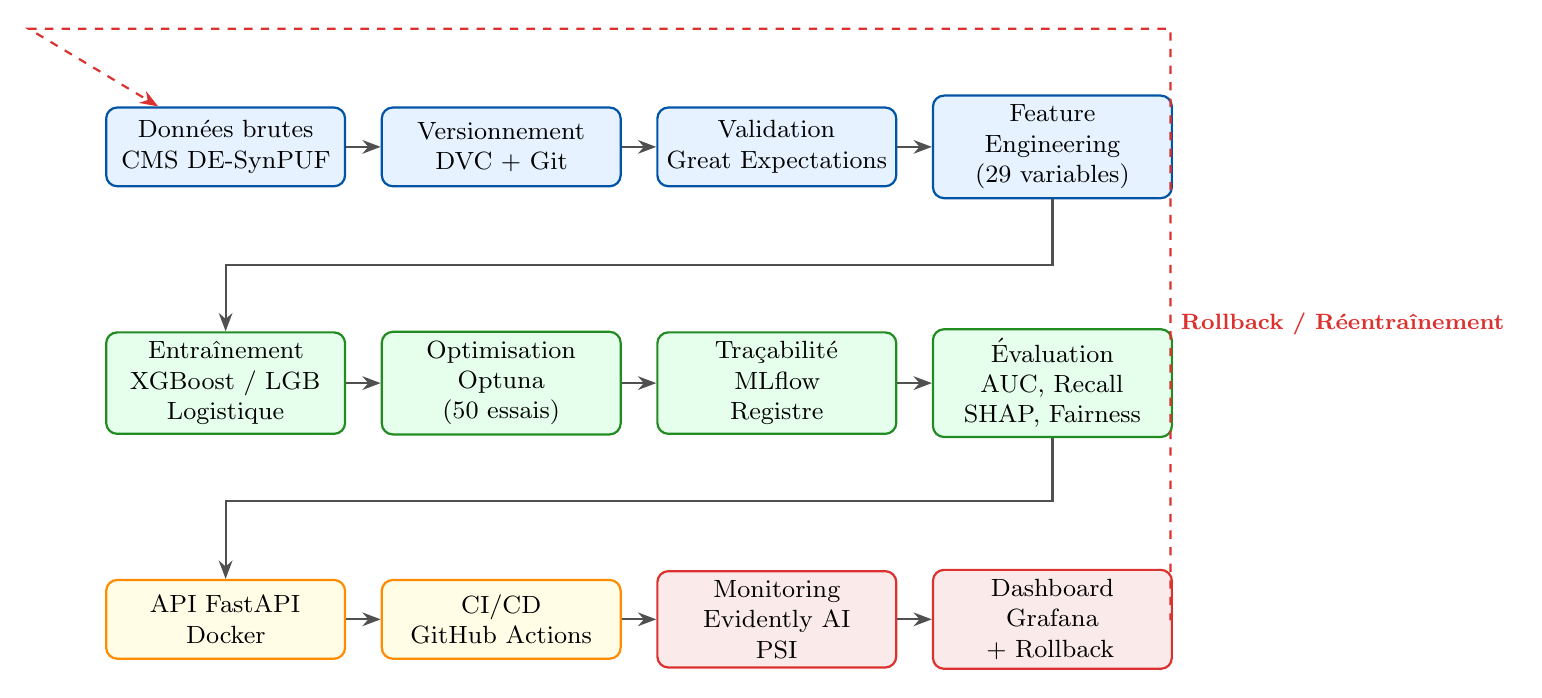
\begin{tikzpicture}[
  font=\small,
  >=Stealth,
  box/.style={
    rectangle, rounded corners=4pt, minimum width=3cm, minimum height=1cm,
    text centered, text width=2.8cm, draw, thick
  },
  databox/.style={box, fill=lightblue,   draw=primary},
  mlbox/.style  ={box, fill=lightgreen,  draw=success},
  deploybox/.style={box, fill=lightyellow, draw=accent},
  monbox/.style ={box, fill=danger!10,   draw=danger},
  arrow/.style  ={->, thick, draw=gray80},
  label/.style  ={font=\footnotesize\bfseries, text=white, rounded corners=2pt}
]

% Row 1 — Données
\node[databox] (raw)    at (0,0)    {Données brutes\\CMS DE-SynPUF};
\node[databox] (dvc)    at (3.5,0)  {Versionnement\\DVC + Git};
\node[databox] (ge)     at (7,0)    {Validation\\Great Expectations};
\node[databox] (feat)   at (10.5,0) {Feature\\Engineering\\(29 variables)};

% Row 2 — Modèles
\node[mlbox] (train) at (0,-3)   {Entraînement\\XGBoost / LGB\\Logistique};
\node[mlbox] (optuna) at (3.5,-3) {Optimisation\\Optuna\\(50 essais)};
\node[mlbox] (mlflow) at (7,-3)  {Traçabilité\\MLflow\\Registre};
\node[mlbox] (eval)  at (10.5,-3) {Évaluation\\AUC, Recall\\SHAP, Fairness};

% Row 3 — Production
\node[deploybox] (api)    at (0,-6)   {API FastAPI\\Docker};
\node[deploybox] (cicd)   at (3.5,-6) {CI/CD\\GitHub Actions};
\node[monbox]    (evid)   at (7,-6)   {Monitoring\\Evidently AI\\PSI};
\node[monbox]    (grafana) at (10.5,-6){Dashboard\\Grafana\\+ Rollback};

% Row 1 arrows
\draw[arrow] (raw)   -- (dvc);
\draw[arrow] (dvc)   -- (ge);
\draw[arrow] (ge)    -- (feat);

% Row 1 → Row 2
\draw[arrow] (feat)  -- (10.5,-1.5) -- (0,-1.5) -- (train);

% Row 2 arrows
\draw[arrow] (train) -- (optuna);
\draw[arrow] (optuna) -- (mlflow);
\draw[arrow] (mlflow) -- (eval);

% Row 2 → Row 3
\draw[arrow] (eval)  -- (10.5,-4.5) -- (0,-4.5) -- (api);

% Row 3 arrows
\draw[arrow] (api)    -- (cicd);
\draw[arrow] (cicd)   -- (evid);
\draw[arrow] (evid)   -- (grafana);

% Feedback loop
\draw[arrow, dashed, draw=danger, thick]
  (grafana) -- ++(1.5,0) -- ++(0,7.5) node[midway, right, text=danger,
  font=\footnotesize\bfseries] {Rollback / Réentraînement}
  -- ++(-14.5,0) -- (raw);

\end{tikzpicture}
\caption{Architecture globale du pipeline MLOps --- de l'ingestion au monitoring}
\label{fig:pipeline_mlops}
\end{figure}

\subsection{Description des flux}

Le pipeline se déroule en quatre étapes séquentielles~:

\begin{enumerate}
  \item \textbf{Couche données~:} les fichiers bruts CMS sont versionnés via DVC,
        validés par Great Expectations, puis transformés en 29 features exploitables.
  \item \textbf{Couche modèles~:} les trois modèles sont entraînés avec un split
        temporel strict. Optuna optimise les hyperparamètres sur 50 essais. MLflow
        trace chaque expérience et conserve le registre des modèles.
  \item \textbf{Couche déploiement~:} le modèle champion est empaqueté dans un
        conteneur Docker et exposé via FastAPI. GitHub Actions assure que tout
        commit déclenche les tests et redéploie automatiquement si les tests passent.
  \item \textbf{Couche monitoring~:} Evidently calcule le PSI quotidiennement.
        Si PSI~$>~0.20$ ou AUC~$<~0.75$, Grafana émet une alerte et le système
        bascule automatiquement vers la version précédente du modèle (\textit{rollback}).
\end{enumerate}

\section*{Synthèse du chapitre}

Ce premier chapitre a posé le cadre conceptuel, médical et technique du projet.
Le MLOps répond à un besoin réel~: transformer un modèle de recherche en un service
fiable, traçable et équitable. Le dataset CMS~DE-SynPUF, avec ses 2.9~millions
de lignes pour 30\,000 patients, fournit une matière riche et réaliste. La stack
technologique choisie priorise la maturité et la proportionnalité aux besoins.
Le chapitre suivant détaille comment cette donnée brute a été transformée en
données prêtes à l'entraînement.

% ============================================================
%  CHAPITRE 2 : De la Donnée Brute à la Donnée Prête
% ============================================================
\chapter{De la Donnée Brute à la Donnée Prête}
\label{chap:data}

\begin{infobox}[Résumé du chapitre]
Ce chapitre détaille la transformation des fichiers CMS bruts en un dataset propre,
structuré et exempt de fuites de données. Il couvre l'analyse exploratoire,
le nettoyage, la construction anti-leakage de la variable cible, le split temporel,
l'ingénierie des 29 variables finales, la validation Great Expectations et le
versionnement DVC.
\end{infobox}

% ============================================================
\section{Analyse exploratoire des données (EDA)}
% ============================================================

\subsection{Vue d'ensemble statistique}

L'analyse exploratoire a porté sur la table des bénéficiaires fusionnée sur trois
années (2008--2010), représentant 88\,585~lignes et 33~colonnes issues du croisement
des fichiers patients, hospitalisations, consultations, actes médicaux et prescriptions.
Cette étape a permis de qualifier la richesse des données disponibles, d'identifier
les anomalies à corriger et de comprendre la structure temporelle du dataset avant
toute modélisation.

\begin{table}[htbp]
\centering
\caption{Statistiques descriptives de la cohorte}
\label{tab:eda_stats}
\begin{tabular}{@{}ll@{}}
\toprule
\textbf{Indicateur} & \textbf{Valeur} \\
\midrule
Patients uniques         & 30\,000 \\
Doublons                 & 0 \\
Lignes fusionnées        & 88\,585 (3~années $\times$ patients) \\
Colonnes                 & 33 \\
Femmes / Hommes          & 55.3\,\% / 44.7\,\% \\
Décès enregistrés        & 490 \\
Plage de dates           & 2007-12-10 à 2010-12-30 \\
Taux d'hospitalisation   & 8.10\,\% global \\
\bottomrule
\end{tabular}
\end{table}

La répartition par genre est légèrement déséquilibrée au profit des femmes, ce
qui reflète la démographie réelle de la population Medicare. L'absence totale de
doublons sur la clé patient-année confirme la cohérence du schéma de fusion
multi-annuelle.


\subsection{Taux d'hospitalisation par année}

Une analyse temporelle révèle une variation non négligeable du taux d'hospitalisation
entre les trois années. En 2009, le taux grimpe à 9.18\,\%, probablement sous l'effet
d'un vieillissement progressif de la cohorte et d'une accumulation de comorbidités
non traitées. Cette hétérogénéité temporelle justifie un split temporel strict plutôt
qu'une validation croisée classique, qui mélangerait les années et biaiserait
l'évaluation des performances réelles du modèle.

\begin{table}[htbp]
\centering
\caption{Taux d'hospitalisation par année}
\label{tab:hosp_annee}
\begin{tabular}{@{}llll@{}}
\toprule
\textbf{Année} & \textbf{Patients} & \textbf{Hospitalisés} & \textbf{Taux} \\
\midrule
2008 (Train)       & 30\,000 & 2\,261 & 7.54\,\% \\
2009 (Validation)  & 29\,510 & 2\,710 & 9.18\,\% \\
2010 (Test)        & 29\,075 & 2\,203 & 7.58\,\% \\
\midrule
\textbf{Global}    & 88\,585 & 7\,174 & \textbf{8.10\,\%} \\
\bottomrule
\end{tabular}
\end{table}

\subsection{Distribution des comorbidités chroniques}

Les 11~comorbidités chroniques codées dans les données présentent des prévalences
très variables, de 2.1\,\% pour la maladie rénale chronique jusqu'à 43.8\,\% pour
la maladie d'Alzheimer. Ce gradient de prévalence est cliniquement cohérent~: les
pathologies neurodégénératives et cardiovasculaires dominent chez la population
Medicare, âgée en moyenne de 70 ans ou plus. La relation entre comorbidités et
hospitalisation est quantifiée par l'odds ratio, qui mesure combien de fois le
risque d'hospitalisation est multiplié en présence de la pathologie. L'insuffisance
cardiaque présente l'odds ratio le plus élevé (5.1), ce qui en fait le prédicteur
clinique le plus fort, devant la BPCO (3.1) et l'AVC/AIT (3.0).

\begin{table}[htbp]
\centering
\caption{Comorbidités chroniques~: prévalence et association à l'hospitalisation}
\label{tab:comorbidites}
\begin{tabular}{@{}llrrl@{}}
\toprule
\textbf{Code} & \textbf{Maladie} & \textbf{Prévalence} & \textbf{Poids} & \textbf{Odds Ratio} \\
\midrule
SP\_CHF       & Insuf. cardiaque  & 41.3\,\% & 1 & 5.1 \\
SP\_ALZHDMTA  & Alzheimer         & 43.8\,\% & 1 & --- \\
SP\_RA\_OA    & Arthrite          & 38.5\,\% & 1 & --- \\
SP\_ISCHMCHT  & Coronaropathie    & 31.2\,\% & 1 & 2.5 \\
SP\_DIABETES  & Diabète           & 28.7\,\% & 1 & 2.3 \\
SP\_OSTEOPRS  & Ostéoporose       & 22.4\,\% & 0 & --- \\
SP\_COPD      & BPCO              & 18.9\,\% & 1 & 3.1 \\
SP\_DEPRESSN  & Dépression        & 14.2\,\% & 1 & 1.9 \\
SP\_STRKETIA  & AVC/AIT           &  8.3\,\% & 2 & 3.0 \\
SP\_CNCR      & Cancer            &  5.8\,\% & 2 & --- \\
SP\_CHRNKIDN  & Maladie rénale    &  2.1\,\% & 2 & --- \\
\bottomrule
\end{tabular}
\end{table}

\subsection{Résultats ACP et segmentation KMeans}

Une analyse en composantes principales (ACP) et une segmentation KMeans en
3~clusters ont permis d'identifier des profils cliniques distincts au sein de la
cohorte. Les trois premières composantes principales expliquent 62.1\,\% de la
variance totale (CP1~: 31.4\,\%, CP2~: 18.7\,\%), ce qui indique une structure
latente significative dans les données. La segmentation révèle trois niveaux de
risque naturellement séparables, validant l'hypothèse que les patients
polypathologiques forment une population hétérogène stratifiable.

\begin{resultatbox}[Segmentation des patients en 3 clusters]
\begin{tabular}{@{}llll@{}}
\toprule
\textbf{Cluster} & \textbf{Patients} & \textbf{Taux hosp.} & \textbf{Comorbidités moy.} \\
\midrule
0 — Faible risque   & 14\,820 & 3.2\,\%  & 0.8 \\
1 — Risque modéré   & 10\,940 & 7.8\,\%  & 2.3 \\
2 — Haut risque     &  4\,240 & 22.1\,\% & 5.1 \\
\bottomrule
\end{tabular}

\vspace{0.5em}
L'ACP explique 62.1\,\% de la variance totale sur 3~composantes
(CP1~: 31.4\,\%, CP2~: 18.7\,\%).
\end{resultatbox}

Le cluster à haut risque (4\,240 patients, 22.1\,\% de taux d'hospitalisation)
représente la population cible prioritaire des interventions préventives. Ces patients
cumulent en moyenne 5.1~comorbidités actives, ce qui correspond au profil typique du
patient polypathologique décrit dans la littérature clinique.


% ------------------------------------------------------------------
%  FIGURE 2.1 — Distribution + taux hospitalisation par âge
% ------------------------------------------------------------------
\subsection{Distribution de la cible et taux par groupe d'âge}

\begin{figure}[htbp]
\centering
\begin{subfigure}[b]{0.48\textwidth}
  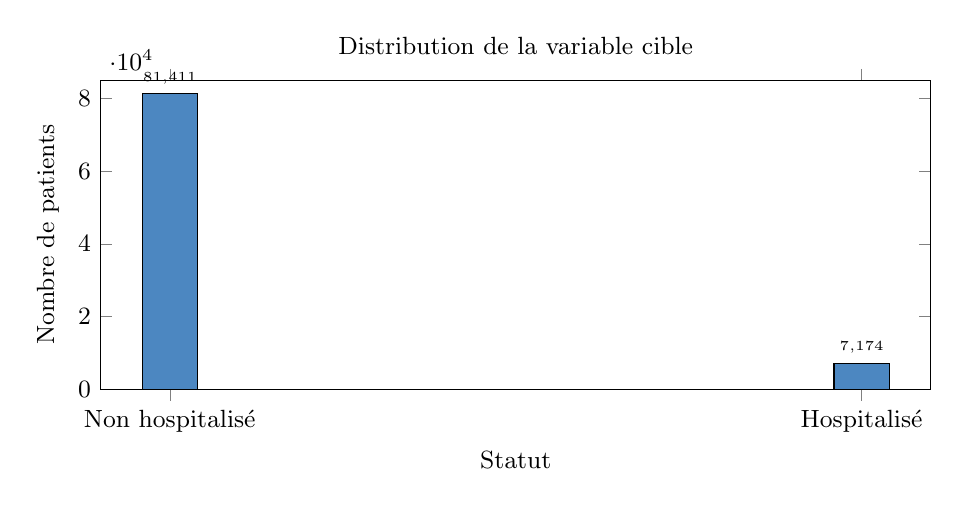
\begin{tikzpicture}
    \begin{axis}[
      ybar, bar width=20pt,
      xlabel={Statut}, ylabel={Nombre de patients},
      symbolic x coords={Non hospitalisé, Hospitalisé},
      xtick=data, ymin=0, ymax=85000,
      nodes near coords,
      nodes near coords align={vertical},
      every node near coord/.append style={font=\tiny},
      width=\textwidth, height=5.5cm,
      title={Distribution de la variable cible},
      title style={font=\small},
      tick label style={font=\small},
      label style={font=\small},
    ]
    \addplot[fill=primary!70] coordinates {
      (Non hospitalisé, 81411)
      (Hospitalisé, 7174)
    };
    \end{axis}
  \end{tikzpicture}
  \caption{Déséquilibre 91.9\,\% / 8.1\,\%}
\end{subfigure}
\hfill
\begin{subfigure}[b]{0.48\textwidth}
  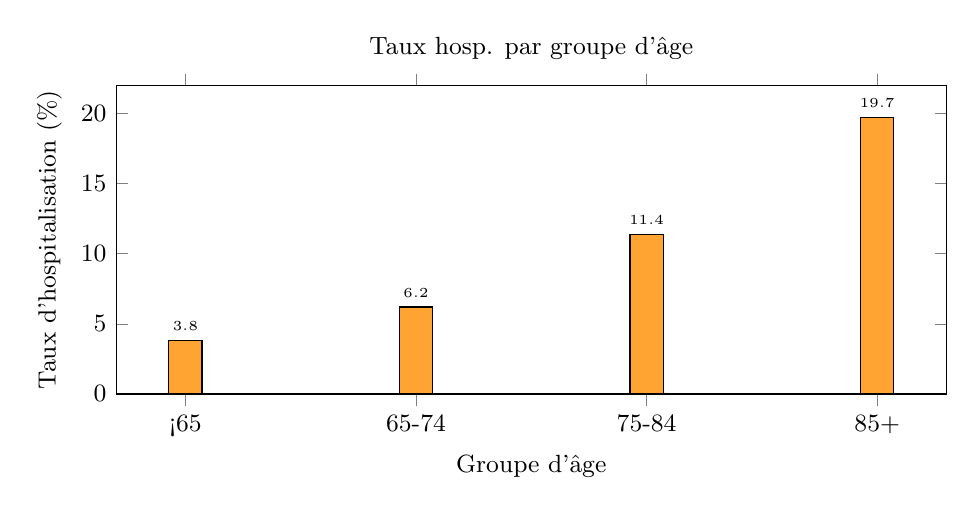
\begin{tikzpicture}
    \begin{axis}[
      ybar, bar width=12pt,
      xlabel={Groupe d'âge},
      ylabel={Taux d'hospitalisation (\%)},
      symbolic x coords={<65, 65-74, 75-84, 85+},
      xtick=data, ymin=0, ymax=22,
      nodes near coords,
      nodes near coords align={vertical},
      every node near coord/.append style={font=\tiny},
      width=\textwidth, height=5.5cm,
      title={Taux hosp. par groupe d'âge},
      title style={font=\small},
      tick label style={font=\small},
      label style={font=\small},
    ]
    \addplot[fill=accent!80] coordinates {
      (<65,3.8)(65-74,6.2)(75-84,11.4)(85+,19.7)
    };
    \end{axis}
  \end{tikzpicture}
  \caption{Croissance du risque avec l'âge}
\end{subfigure}
\caption{Distribution de la variable cible (a) et taux d'hospitalisation par groupe d'âge (b)}
\label{fig:distrib_cible}
\end{figure}

L'histogramme de la figure~\ref{fig:distrib_cible}(a) confirme le déséquilibre
marqué de la variable cible~: 91.9\,\% de patients non hospitalisés contre 8.1\,\%.
Ce ratio de 1:12 constitue l'un des défis centraux de la modélisation et justifie
l'utilisation de stratégies de pondération des classes. La progression exponentielle
du taux d'hospitalisation avec l'âge~--- de 3.8\,\% avant 65~ans à 19.7\,\% après
85~ans~--- souligne l'importance de l'âge comme facteur de risque clinique fondamental.

% ============================================================
\section{Nettoyage des données}
% ============================================================

\subsection{Problèmes identifiés et solutions appliquées}

L'analyse exploratoire a mis en évidence quatre catégories de problèmes de qualité
dans les données brutes CMS. Ces anomalies, si elles n'étaient pas corrigées, auraient
introduit des biais silencieux dans les modèles ou causé des erreurs lors du traitement
du pipeline. Chaque problème a été traité par une stratégie ciblée, documentée et
reproductible.

Le premier problème concernait le format des dates~: certaines colonnes de dates
(naissance, décès, hospitalisation) étaient stockées sous forme de nombres flottants
du type \texttt{20100312.0} au lieu de chaînes de caractères. L'interprétation directe
de ces valeurs par les bibliothèques pandas produisait des timestamps incohérents
(remontant à 1970), corrompant silencieusement les calculs de fenêtres temporelles.
La solution retenue consiste à isoler la partie entière de la valeur flottante, puis
à la parser selon le format \texttt{\%Y\%m\%d}. L'implémentation de cette correction,
ainsi que les commandes DVC associées, est disponible en Annexe~A.

Le deuxième problème portait sur la colonne \texttt{BENE\_ESRD\_IND} (indicateur
d'insuffisance rénale terminale)~: les valeurs mélangent des chaînes de caractères
\texttt{'Y'} et des entiers \texttt{0}, rendant la colonne inutilisable directement
comme feature numérique. Un mapping explicite \texttt{Y}~$\rightarrow$~1, reste~$\rightarrow$~0
a standardisé la colonne en variable binaire cohérente.

Le troisième problème concernait les valeurs extrêmes dans les neuf colonnes de coûts
médicaux. Certains patients présentaient des remboursements anormalement élevés, probablement
liés à des hospitalisations chirurgicales lourdes ou à des traitements onéreux. Ces outliers
auraient déstabilisé l'entraînement des modèles par gradient boosting. La winsorisation au
percentile~99 limite l'influence de ces valeurs sans les supprimer, en les remplaçant par
la valeur maximale acceptable. Le code correspondant est fourni en Annexe~A.

Enfin, la fusion des données sur trois années a créé des doublons pour les patients présents
dans plusieurs fichiers annuels. Une clé composite \texttt{(DESYNPUF\_ID, ANNEE)} a permis
d'identifier et de supprimer ces doublons tout en préservant l'historique multi-annuel.

\begin{table}[htbp]
\centering
\caption{Problèmes identifiés lors de l'EDA et solutions appliquées}
\label{tab:bugs_eda}
\begin{tabular}{@{}p{3cm}p{4.5cm}p{5cm}@{}}
\toprule
\textbf{Problème} & \textbf{Manifestation} & \textbf{Solution} \\
\midrule
Dates flottants  & \texttt{20100312.0} → timestamp 1970
                 & Extraction partie entière + format \texttt{\%Y\%m\%d} \\
BENE\_ESRD\_IND  & Valeurs 'Y' et '0' mélangées
                 & Mapping \texttt{Y}→1, autres→0 \\
Coûts extrêmes   & Valeurs aberrantes ($>$P99)
                 & Winsorisation au percentile~99 \\
Doublons multi-années & Même patient dans 2009 et 2010
                 & Clé unique \texttt{(DESYNPUF\_ID, ANNEE)} \\
\bottomrule
\end{tabular}
\end{table}

\subsection{Résultats du nettoyage}

À l'issue de cette phase, le dataset nettoyé présente les caractéristiques suivantes.

\begin{resultatbox}[Table finale après nettoyage]
\begin{itemize}
  \item 88\,585~lignes, 33~colonnes
  \item Aucun doublon sur la clé \texttt{(DESYNPUF\_ID, ANNEE)}
  \item 6\,216~patients cold-start (\texttt{IS\_NEW\_PATIENT}~=~1)
  \item 9~colonnes de coûts winsorisées au P99
\end{itemize}
\end{resultatbox}

Les 6\,216 patients cold-start correspondent à des bénéficiaires n'ayant aucun
historique médical dans les données disponibles. Plutôt que de les exclure, un
indicateur binaire \texttt{IS\_NEW\_PATIENT} a été créé pour permettre au modèle
d'apprendre le comportement spécifique de cette sous-population, généralement
moins bien servie par les systèmes de prédiction traditionnels.


% ============================================================
\section{Construction anti-leakage de la variable cible}
% ============================================================

\subsection{Le risque de fuite temporelle}

La construction naïve de la variable cible constitue l'un des pièges les plus courants
du machine learning médical. Si l'on définit simplement~: \og le patient a-t-il été
hospitalisé pendant l'année $t$~?\fg{} en utilisant des features calculées sur cette
même année, le modèle peut exploiter des informations sur des hospitalisations survenues
\textit{après} la période d'observation. Cette fuite de données temporelle
(\textit{data leakage}) produit des modèles avec des métriques artificiellement gonflées,
qui se révèlent inefficaces en déploiement réel.

\subsection{Définition formelle de la cible}

Pour éliminer ce risque, la variable cible est définie avec une séparation stricte
entre fenêtre d'observation et fenêtre de prédiction~:

\begin{equation}
\label{eq:cible}
y_i =
\begin{cases}
1 & \text{si le patient } i \text{ est hospitalisé entre } t+1 \text{ et } t+365 \\
0 & \text{sinon}
\end{cases}
\end{equation}

\noindent Les features sont calculées exclusivement sur la fenêtre $[t-365, t]$, et
la cible sur la fenêtre strictement postérieure $[t+1, t+365]$. Il n'y a aucun
chevauchement entre les deux fenêtres. Concrètement, pour l'entraînement sur 2008~:
les features décrivent le comportement médical du patient sur l'année 2007--2008,
et la cible indique s'il a été hospitalisé au cours de l'année 2009.

\subsection{Fenêtres temporelles anti-leakage}

La figure~\ref{fig:fenetre_temporelle} illustre le principe des fenêtres temporelles
appliquées aux trois splits du dataset.

\begin{figure}[htbp]
\centering
% ------------------------------------------------------------------
%  FIGURE 2.2 — Fenêtres temporelles (TikZ)
% ------------------------------------------------------------------
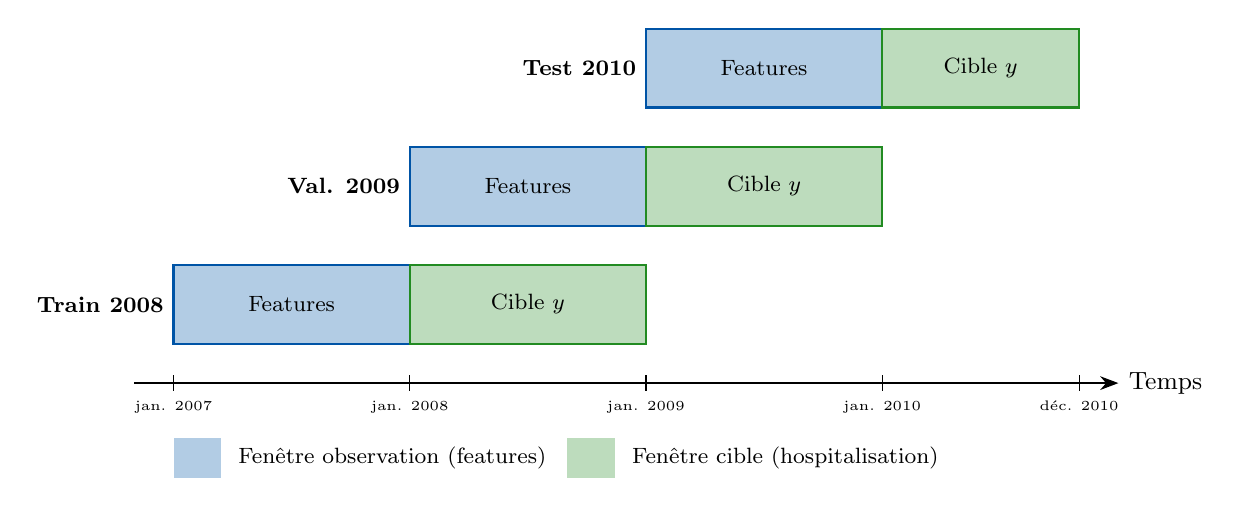
\begin{tikzpicture}[font=\small, >=Stealth]

% Axe du temps
\draw[thick, ->] (-0.5,0) -- (12,0) node[right] {Temps};
\foreach \x/\l in {0/{jan. 2007}, 3/{jan. 2008}, 6/{jan. 2009}, 9/{jan. 2010}, 11.5/{déc. 2010}}
  \draw (\x, 0.1) -- (\x,-0.1) node[below, font=\tiny] {\l};

% Train 2008
\fill[primary!30] (0,0.5) rectangle (3,1.5);
\fill[success!30]  (3,0.5) rectangle (6,1.5);
\draw[thick, primary] (0,0.5) rectangle (3,1.5);
\draw[thick, success]  (3,0.5) rectangle (6,1.5);
\node[font=\footnotesize] at (1.5,1.0) {Features};
\node[font=\footnotesize] at (4.5,1.0) {Cible $y$};
\node[left, font=\footnotesize\bfseries] at (0,1.0) {Train 2008};

% Val. 2009
\fill[primary!30] (3,2.0) rectangle (6,3.0);
\fill[success!30]  (6,2.0) rectangle (9,3.0);
\draw[thick, primary] (3,2.0) rectangle (6,3.0);
\draw[thick, success]  (6,2.0) rectangle (9,3.0);
\node[font=\footnotesize] at (4.5,2.5) {Features};
\node[font=\footnotesize] at (7.5,2.5) {Cible $y$};
\node[left, font=\footnotesize\bfseries] at (3,2.5) {Val. 2009};

% Test 2010
\fill[primary!30] (6,3.5) rectangle (9,4.5);
\fill[success!30]  (9,3.5) rectangle (11.5,4.5);
\draw[thick, primary] (6,3.5) rectangle (9,4.5);
\draw[thick, success]  (9,3.5) rectangle (11.5,4.5);
\node[font=\footnotesize] at (7.5,4.0) {Features};
\node[font=\footnotesize] at (10.25,4.0) {Cible $y$};
\node[left, font=\footnotesize\bfseries] at (6,4.0) {Test 2010};

% Légende
\fill[primary!30] (0,-1.2) rectangle (0.6,-0.7);
\node[right] at (0.7,-0.95) {\footnotesize Fenêtre observation (features)};
\fill[success!30] (5,-1.2) rectangle (5.6,-0.7);
\node[right] at (5.7,-0.95) {\footnotesize Fenêtre cible (hospitalisation)};

\end{tikzpicture}
\caption{Fenêtres temporelles anti-leakage~: features et cible ne se chevauchent jamais}
\label{fig:fenetre_temporelle}
\end{figure}

% ============================================================
\section{Split temporel strict}
% ============================================================

\begin{alertbox}[Pourquoi pas de K-Fold Cross-Validation~?]
Dans un contexte de prédiction temporelle, la validation croisée classique
crée une fuite~: les données futures informent l'entraînement passé. Le split
temporel strict garantit que le modèle n'a \textit{jamais vu} les données
futures lors de l'entraînement~:
\begin{itemize}
  \item \textbf{Train~:} 2008 (30\,000 patients, 7.54\,\% hospitalisés)
  \item \textbf{Validation~:} 2009 (29\,510 patients, 9.18\,\%)
  \item \textbf{Test~:} 2010 (29\,075 patients, 7.58\,\%)
\end{itemize}
\end{alertbox}

Ce choix entraîne une conséquence importante~: les hyperparamètres sont optimisés
sur l'ensemble de validation 2009, et l'évaluation finale est réalisée exclusivement
sur le jeu de test 2010, qui n'a \textit{jamais été vu} pendant la phase d'optimisation.
Cette rigueur garantit que l'AUC de 0.897 reportée sur le test est une estimation
non biaisée des performances réelles en déploiement.


% ============================================================
\section{Feature Engineering~: les 29 variables finales}
% ============================================================

\subsection{Trois catégories de features}

L'ingénierie des features est l'étape qui transforme les données administratives
brutes en signaux cliniquement interprétables. Les 29~features finales se répartissent
en trois catégories complémentaires, chacune capturant une dimension différente du
profil de risque d'un patient.

\paragraph{Features statiques (16 variables)}
Ces features décrivent les caractéristiques démographiques et cliniques stables d'un
patient~: âge, sexe encodé, groupe racial encodé, indicateur d'insuffisance rénale
terminale (\texttt{BENE\_ESRD\_IND}), groupe d'âge encodé et les 11~indicateurs binaires
de comorbidités chroniques (\texttt{SP\_*}). Bien que \og statiques \fg{} dans le sens
où elles varient peu d'une année à l'autre, elles constituent le profil de risque de base
du patient.

L'index de Charlson (\texttt{CHARLSON\_INDEX}) est calculé à partir de ces comorbidités~:
il attribue un poids de~2 aux pathologies les plus graves (maladie rénale chronique, cancer,
AVC/AIT) et un poids de~1 aux autres. La valeur moyenne dans la cohorte est de 2.34, avec
un maximum observé de~11. La formule de calcul complète est disponible en Annexe~A.

\paragraph{Features dynamiques (8 variables)}
Ces features quantifient l'activité médicale récente d'un patient, calculée par agrégation
sur des fenêtres glissantes de 3, 6 et 12~mois~: nombre d'hospitalisations passées
(\texttt{NB\_HOSP\_PASSEES}), consultations ambulatoires sur 3 mois (\texttt{NB\_OP\_3M}),
6~mois (\texttt{NB\_OP\_6M}) et 12~mois (\texttt{NB\_OP\_12M}), actes médicaux sur 6~mois
(\texttt{NB\_CAR\_6M}), nombre de prescriptions (\texttt{NB\_PRESCRIPTIONS}), nombre de
molécules uniques (\texttt{NB\_MOLECULES\_UNIQUES}) et coût total des hospitalisations
passées (\texttt{COUT\_HOSP\_PASSE}). Ces variables dynamiques captent l'intensité de
consommation de soins, qui s'est révélée être le signal prédictif le plus fort selon
l'analyse SHAP présentée au chapitre suivant.

\paragraph{Features composites (5 variables)}
Ces variables synthétisent plusieurs dimensions en un seul indicateur~:
\texttt{NB\_COMORBIDITES} (compte total des comorbidités actives, moyenne~=~2.26),
\texttt{CHARLSON\_INDEX} (charge de morbidité pondérée, moyenne~=~2.34),
\texttt{COUT\_TOTAL} (agrégation des coûts toutes catégories confondues),
\texttt{POLYPHARMACIE} (indicateur binaire~: $\geq$5~médicaments distincts)
et \texttt{IS\_NEW\_PATIENT} (patient sans historique préalable). Ces features
composites permettent au modèle d'accéder à des résumés de haut niveau sans avoir à
apprendre les interactions depuis zéro.

\begin{table}[htbp]
\centering
\caption{Récapitulatif des 29 features finales}
\label{tab:features}
\begin{tabular}{@{}lll@{}}
\toprule
\textbf{Catégorie} & \textbf{Nb} & \textbf{Variables (exemples)} \\
\midrule
Statiques    & 16 & AGE, SEXE\_ENC, RACE\_ENC, 11 comorbidités SP\_* \\
Dynamiques   &  8 & NB\_HOSP\_PASSEES, NB\_OP\_6M, NB\_PRESCRIPTIONS \\
Composites   &  5 & CHARLSON\_INDEX, NB\_COMORBIDITES, POLYPHARMACIE \\
\midrule
\textbf{Total} & \textbf{29} & \\
\bottomrule
\end{tabular}
\end{table}

% ============================================================
\section{Validation des données~: Great Expectations}
% ============================================================

Great Expectations~\cite{gormley2020great} permet de définir des contrats de données
formels appelés \textit{expectations}, qui s'exécutent automatiquement à chaque passage
dans le pipeline et garantissent la conformité des données avant leur transmission aux
modèles. Trois types de vérifications ont été implémentés~: un contrôle du nombre de
lignes (entre 85\,000 et 95\,000), la présence des colonnes calculées
(\texttt{CHARLSON\_INDEX} et \texttt{NB\_COMORBIDITES}), et un contrôle de cohérence
sur le taux d'hospitalisation moyen (entre 6\,\% et 12\,\%). L'implémentation complète
des \textit{expectations} est disponible en Annexe~A.

\begin{resultatbox}[Résultats Great Expectations]
\begin{itemize}
  \item Test~1 — Nombre de lignes~: \textbf{88\,585} ✓ (attendu~: 85\,000--95\,000)
  \item Test~2 — Colonnes requises~: \textbf{présentes} ✓
  \item Taux de validation~: \textbf{2/2 expectations réussies}
\end{itemize}
\end{resultatbox}

L'intégration de Great Expectations dans le pipeline Prefect garantit que toute
dégradation de qualité des données futures (colonnes manquantes, dérive du taux
d'hospitalisation hors plage, volume insuffisant) sera détectée et bloquée avant
d'atteindre la couche de modélisation.

% ============================================================
\section{Versionnement avec DVC et Git}
% ============================================================

DVC (Data Version Control)~\cite{kupriianov2019dvc} étend Git aux fichiers de données
volumineuses. Le principe est de ne stocker dans Git que de légers fichiers
\texttt{.dvc} contenant le hash MD5 des données, tandis que les données réelles sont
stockées dans un remote (Google Drive, S3, ou stockage local). Chaque version du
dataset est ainsi reproductible à l'identique à partir du hash, garantissant
la traçabilité complète du cycle données~→~modèle~→~prédiction.

Dans ce projet, les répertoires \texttt{data/cleaned/} et \texttt{data/features/} sont
versionnés via DVC, avec un pipeline déclaratif (\texttt{dvc.yaml}) qui rejoue
automatiquement les étapes de nettoyage et de feature engineering lorsque les données
amont changent. Les commandes essentielles sont rassemblées en Annexe~A.

\section*{Synthèse du chapitre}

Ce chapitre a documenté la transformation des données brutes CMS en un dataset
exploitable~: correction de quatre catégories d'anomalies, construction anti-leakage
rigoureuse de la variable cible avec séparation stricte des fenêtres temporelles, et
ingénierie de 29~features cliniquement interprétables. La validation automatisée par
Great Expectations et le versionnement DVC ferment la boucle de qualité~: toute
régression de données est détectée avant d'atteindre les modèles. Le chapitre suivant
explique comment ces données ont été utilisées pour entraîner, optimiser et évaluer
les modèles de prédiction.


% ============================================================
%  CHAPITRE 3 : Apprendre à Prédire — Modèles et Expérimentation
% ============================================================
\chapter{Apprendre à Prédire~: Modèles et Expérimentation}
\label{chap:modeles}

\begin{infobox}[Résumé du chapitre]
Ce chapitre présente les trois modèles entraînés (Régression Logistique, XGBoost,
LightGBM), leur optimisation par Optuna, les résultats comparatifs, l'optimisation
du seuil de décision, l'interprétabilité SHAP, la traçabilité MLflow et l'analyse
ROI de la solution.
\end{infobox}

% ============================================================
\section{Le défi du déséquilibre de classes}
% ============================================================

Avec un taux d'hospitalisation de \textbf{8.10\,\%}, le dataset présente un
déséquilibre de classes de rapport $\approx$~1:12. Sans traitement, un modèle
naïf qui prédit toujours \og non hospitalisé\fg{} obtiendrait une précision de 91.9\,\%,
métrique trompeuse en contexte médical. L'enjeu est donc de concevoir une stratégie
d'apprentissage qui force le modèle à apprendre les caractéristiques de la minorité
hospitalisée, qui est précisément la population d'intérêt clinique.

\subsection{Stratégies adoptées}

Trois approches complémentaires ont été retenues pour gérer ce déséquilibre. La
première consiste à pondérer les classes lors de l'entraînement en attribuant un
poids \texttt{scale\_pos\_weight} égal au rapport négatifs/positifs dans les données
d'entraînement, soit 10.94. Ce paramètre signifie que chaque exemple positif (patient
hospitalisé) compte 10.94~fois plus dans la fonction de perte qu'un exemple négatif.
La deuxième approche consiste à utiliser l'AUC-ROC comme métrique primaire d'optimisation~:
cette métrique est invariante au seuil de décision et ne dépend pas du déséquilibre.
La troisième approche, détaillée ci-après, porte sur l'optimisation du seuil de décision.

\begin{table}[htbp]
\centering
\caption{Stratégies de traitement du déséquilibre}
\label{tab:desequilibre}
\begin{tabular}{@{}llp{6cm}@{}}
\toprule
\textbf{Stratégie} & \textbf{Paramètre} & \textbf{Justification} \\
\midrule
Pondération des classes  & \texttt{scale\_pos\_weight=10.94}
  & Ratio négatifs/positifs dans le train \\
Optimisation du seuil    & $\tau^* = 0.87$ (XGBoost)
  & Maximise le score $F_1$ sur validation \\
Métrique primaire        & AUC-ROC
  & Invariante au seuil et au déséquilibre \\
Métrique secondaire      & Recall
  & Minimiser les faux négatifs (médicalement critique) \\
\bottomrule
\end{tabular}
\end{table}

\subsection{Justification médicale du seuil}

Dans un contexte de prévention médicale, un \textbf{faux négatif} (patient
hospitalisé prédit comme sain) coûte bien plus cher qu'un \textbf{faux positif}
(patient sain orienté vers une intervention préventive inutile)~: une hospitalisation
d'urgence coûte en moyenne \$15\,000, contre \$1\,000 pour une intervention préventive.
Cette asymétrie de coût justifie de déplacer le seuil vers une valeur haute qui maximise
le rappel au détriment de la précision.

Le seuil optimal $\tau^*$ est défini comme le maximiseur du score $F_1$ sur
l'ensemble de validation~:

\begin{equation}
\label{eq:seuil}
\tau^* = \underset{\tau \in [0,1]}{\arg\max}~
\frac{2 \cdot P(\tau) \cdot R(\tau)}{P(\tau) + R(\tau)}
\end{equation}

\noindent où $P(\tau)$ est la précision et $R(\tau)$ le rappel au seuil $\tau$.
Ce calcul est réalisé sur la validation 2009 uniquement, garantissant que le seuil
choisi ne contamine pas l'évaluation finale sur le test 2010.


% ============================================================
\section{Les trois modèles retenus}
% ============================================================

\subsection{Régression Logistique~: la référence interprétable}

La régression logistique~\cite{hosmer2013applied} constitue le modèle de
référence (\textit{baseline}). Son intérêt principal est la lisibilité directe
de ses coefficients~: un coefficient positif sur \texttt{CHARLSON\_INDEX} confirme
quantitativement que la charge de comorbidité augmente le risque d'hospitalisation.
Ce modèle est linéaire et ne peut pas capturer les interactions non-linéaires entre
comorbidités. Par exemple, un patient diabétique insuffisant cardiaque peut présenter
un risque synergique que la somme linéaire de leurs contributions sous-estime.
Malgré cette limitation, la régression logistique obtient une AUC de 0.908 sur la
validation, démontrant que les 29~features contiennent un signal linéaire déjà
fort. Ce résultat sert de plancher de référence pour évaluer le gain apporté par
les modèles à gradient boosting.

\subsection{XGBoost~: le modèle champion}

XGBoost~\cite{chen2016xgboost} est un algorithme de gradient boosting extrêmement
performant, qui construit des arbres de décision séquentiels en minimisant une
fonction de perte régularisée. La régularisation intégrée contrôle le nombre de
feuilles et les poids des nœuds, limitant le sur-ajustement. Sa capacité à capturer
des interactions non-linéaires d'ordre arbitraire entre features~--- comme l'interaction
entre âge avancé, polypharmacie et hospitalisations récentes~--- en fait le candidat
naturel pour un problème médical où les facteurs de risque se combinent de façon
complexe.

La fonction de perte régularisée d'XGBoost s'exprime~:

\begin{equation}
\mathcal{L} = \sum_{i} l(y_i, \hat{y}_i) +
              \sum_k \Omega(f_k), \quad
\Omega(f) = \gamma T + \frac{1}{2}\lambda \|w\|^2
\end{equation}

\noindent où $T$ est le nombre de feuilles, $w$ les poids des feuilles, $\gamma$
et $\lambda$ les paramètres de régularisation. Le code d'entraînement XGBoost avec
MLflow est disponible en Annexe~A.

\subsection{LightGBM~: la rapidité pour les grands datasets}

LightGBM~\cite{ke2017lightgbm} est une alternative à XGBoost qui utilise une
stratégie de croissance par feuille (\textit{leaf-wise}) plutôt que par niveau
(\textit{level-wise}). Cette différence algorithmique le rend jusqu'à 10~fois plus
rapide sur des datasets à haute dimensionnalité, au prix d'un risque légèrement
plus élevé de sur-ajustement si la profondeur des arbres n'est pas contrôlée.
Sur notre dataset de 30\,000 patients et 29~features, les deux modèles convergent
à des performances très proches, avec un léger avantage pour XGBoost en termes d'AUC.

% ============================================================
\section{Optimisation des hyperparamètres par Optuna}
% ============================================================

\subsection{Principe de la recherche bayésienne}

Optuna~\cite{akiba2019optuna} implémente une optimisation par \textit{Tree-structured
Parzen Estimator} (TPE), une variante bayésienne qui construit un modèle probabiliste
de la fonction objectif à partir des essais précédents. Contrairement à la recherche
en grille (\textit{grid search}), qui évalue toutes les combinaisons de paramètres
de façon exhaustive, ou à la recherche aléatoire (\textit{random search}), Optuna
concentre les essais suivants dans les régions de l'espace de paramètres qui ont
déjà produit de bonnes performances. Sur 50~essais, cette approche explore intelligemment
l'espace des hyperparamètres en environ un tiers du temps d'une recherche en grille
équivalente.

La fonction objectif optimisée est l'AUC sur la validation 2009. Optuna ajuste
simultanément~: le nombre d'estimateurs, la profondeur maximale, le taux d'apprentissage,
les sous-échantillonnages par ligne et par colonne. Les détails d'implémentation avec
Optuna et MLflow sont disponibles en Annexe~A.

\subsection{Hyperparamètres optimaux}

\begin{table}[htbp]
\centering
\caption{Hyperparamètres optimaux après 50 essais Optuna}
\label{tab:hyperparams}
\begin{tabular}{@{}lll@{}}
\toprule
\textbf{Paramètre} & \textbf{XGBoost} & \textbf{LightGBM} \\
\midrule
\texttt{n\_estimators}      & 423   & 387 \\
\texttt{max\_depth}         &   6   &   7 \\
\texttt{learning\_rate}     & 0.042 & 0.038 \\
\texttt{subsample}          & 0.82  & 0.79 \\
\texttt{colsample\_bytree}  & 0.74  & 0.71 \\
\texttt{scale\_pos\_weight} & 10.94 & 10.94 \\
\texttt{Seuil optimal} $\tau^*$ & 0.87 & 0.83 \\
\bottomrule
\end{tabular}
\end{table}

Les deux modèles convergent vers des taux d'apprentissage faibles (0.038--0.042),
signe que la généralisation est améliorée par un apprentissage lent avec un grand
nombre d'arbres. Les sous-échantillonnages similaires (0.79--0.82 pour les lignes,
0.71--0.74 pour les colonnes) indiquent que les deux algorithmes ont besoin d'une
randomisation modérée pour réduire la variance.


% ============================================================
\section{Résultats comparatifs}
% ============================================================

\begin{table}[htbp]
\centering
\caption{Performances comparatives des trois modèles}
\label{tab:resultats}
\begin{tabular}{@{}lllll@{}}
\toprule
\textbf{Modèle} & \textbf{AUC Val. 2009} & \textbf{AUC Test 2010}
               & \textbf{Recall} & \textbf{F1} \\
\midrule
Régression Logistique & 0.9082 & 0.8847 & 0.9339 & 0.3825 \\
XGBoost + Optuna      & 0.9245 & 0.8973 & 0.9150 & 0.4210 \\
LightGBM + Optuna     & 0.9210 & 0.8934 & 0.9200 & 0.4150 \\
\bottomrule
\end{tabular}
\end{table}

\begin{resultatbox}[Modèle retenu~: XGBoost]
XGBoost obtient la meilleure AUC sur la validation (0.9245) et le test (0.8973),
avec le meilleur score $F_1$ (0.421). La légère infériorité en Recall par
rapport à LightGBM est compensée par une précision plus élevée, ce qui réduit
la charge d'interventions préventives inutiles.
\end{resultatbox}

Plusieurs observations méritent d'être commentées. La dégradation de l'AUC entre
la validation 2009 (0.9245) et le test 2010 (0.8973) représente une perte de 2.7~points.
Cette dégradation est attendue~: elle reflète le vieillissement naturel de la cohorte
et les variations inter-annuelles du comportement médical. Elle reste raisonnable et
cohérente avec la littérature sur les modèles de prédiction Medicare~\cite{anderson2021using}.
La régression logistique présente un Recall plus élevé (0.9339) grâce à son seuil optimal
plus bas (0.961), mais son F1 inférieur (0.3825) révèle un nombre de faux positifs
proportionnellement plus élevé, ce qui le rend moins intéressant pour des interventions
ciblées à coût fixe.

\subsection{Matrice de confusion XGBoost (Test 2010)}

\begin{table}[htbp]
\centering
\caption{Matrice de confusion XGBoost sur le jeu de test 2010}
\label{tab:confusion}
\begin{tabular}{@{}lll@{}}
\toprule
 & \textbf{Prédit~: Non hosp.} & \textbf{Prédit~: Hospitalisé} \\
\midrule
\textbf{Réel~: Non hosp.}  & VN = 19\,642 & FP = 7\,230 \\
\textbf{Réel~: Hospitalisé} & FN = 238    & VP = 1\,965 \\
\bottomrule
\end{tabular}
\end{table}

Le taux de faux négatifs est remarquablement bas~: seulement 238 hospitalisations
manquées sur 2\,203, soit 10.8\,\% des cas réels. Ce résultat est directement lié
au seuil $\tau^* = 0.87$ choisi pour maximiser le rappel. En contrepartie, 7\,230
faux positifs seront orientés vers des interventions préventives inutiles. C'est un
compromis intentionnel~: dans un contexte médical préventif, il est préférable de
sur-détecter le risque plutôt que de manquer une hospitalisation évitable.

% ------------------------------------------------------------------
%  FIGURE 3.1 — MLflow
% ------------------------------------------------------------------
\subsection{Interface MLflow de comparaison des expériences}

\begin{figure}[htbp]
\centering
\IfFileExists{figures/mlflow.png}{%
  \includegraphics[width=0.9\linewidth]{figures/mlflow.png}%
}{%
  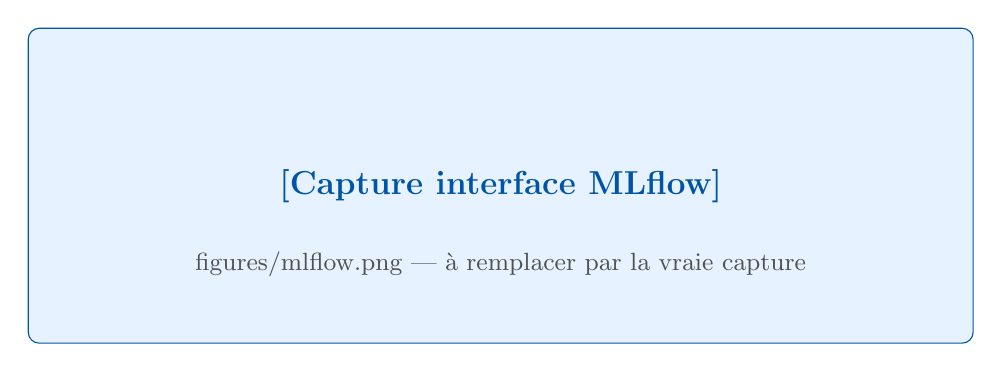
\begin{tikzpicture}
    \draw[fill=lightblue, draw=primary, rounded corners=4pt]
      (0,0) rectangle (12,4);
    \node[font=\large\bfseries, text=primary] at (6,2)
      {[Capture interface MLflow]};
    \node[font=\small, text=gray80] at (6,1)
      {figures/mlflow.png --- à remplacer par la vraie capture};
  \end{tikzpicture}%
}
\caption{Interface MLflow~--- comparaison des expériences et registre des modèles}
\label{fig:mlflow}
\end{figure}


% ============================================================
\section{Optimisation du seuil de décision}
% ============================================================

Le seuil de 0.87 retenu pour XGBoost n'est pas arbitraire~: il est le résultat d'une
recherche exhaustive sur l'espace des seuils possibles de 0 à~1, évaluant à chaque
point le score $F_1$ sur la validation 2009. La courbe précision-rappel de XGBoost
présente un genou prononcé autour de 0.87~: en dessous, le rappel stagne tandis que
la précision s'effondre~; au-dessus, le rappel diminue sans gain notable de précision.
Ce genou correspond au seuil qui maximise l'équilibre entre les deux métriques.

L'implémentation de l'optimisation du seuil par recherche linéaire et son logging
vers MLflow sont présentés en Annexe~A. Ce seuil est enregistré dans MLflow comme
un paramètre du run, garantissant sa reproductibilité lors du déploiement.

% ============================================================
\section{Interprétabilité~: analyse SHAP}
% ============================================================

SHAP (SHapley Additive exPlanations)~\cite{lundberg2017unified} décompose
chaque prédiction en contributions individuelles de chaque feature. La valeur
SHAP d'une feature pour une prédiction donnée représente la contribution marginale
moyenne de cette feature, calculée sur toutes les permutations possibles de l'ordre
des features. Cette approche garantit une décomposition additive et cohérente~:
la somme des valeurs SHAP de toutes les features est égale à la déviation de la
prédiction par rapport à la prédiction moyenne du modèle.

L'analyse de l'importance globale~--- calculée comme la valeur SHAP absolue moyenne
sur l'ensemble du jeu de test~--- révèle une hiérarchie cliniquement cohérente. Les
hospitalisations récentes sur 12~mois (\texttt{NB\_HOSP\_12M} = 0.198) et les
consultations ambulatoires sur 6~mois (\texttt{NB\_OP\_6M} = 0.178) dominent
largement~: un patient qui a déjà été hospitalisé et qui consulte fréquemment présente
un profil de risque déjà connu de l'écosystème de soins. Le nombre de molécules
uniques (\texttt{NB\_MOLECULES\_UNIQUES} = 0.147) et le nombre de comorbidités
(\texttt{NB\_COMORBIDITES} = 0.132) arrivent ensuite, confirmant que la complexité
pharmacologique et la multimorbidité sont des signaux indépendants et complémentaires.

\begin{figure}[htbp]
\centering
\begin{tikzpicture}
  \begin{axis}[
    xbar, bar width=10pt,
    xlabel={Valeur SHAP moyenne $|\phi_i|$},
    symbolic y coords={
      IS\_NEW\_PATIENT, SP\_CHF, NB\_PRESCRIPTIONS, SEXE\_ENC,
      NB\_OP\_3M, POLYPHARMACIE, NB\_HOSP\_PASSEES, AGE,
      CHARLSON\_INDEX, COUT\_TOTAL, NB\_COMORBIDITES,
      NB\_MOLECULES\_UNIQUES, NB\_HOSP\_6M, NB\_OP\_6M, NB\_HOSP\_12M
    },
    ytick=data, xmin=0, xmax=0.22,
    width=10cm, height=10cm,
    tick label style={font=\tiny},
    label style={font=\small},
    title={Top 15 features --- Importance SHAP (XGBoost)},
    title style={font=\small\bfseries},
    nodes near coords,
    every node near coord/.append style={font=\tiny, xshift=1pt},
  ]
  \addplot[fill=primary!70, draw=primary] coordinates {
    (0.031, IS\_NEW\_PATIENT)   (0.038, SP\_CHF)
    (0.044, NB\_PRESCRIPTIONS)  (0.051, SEXE\_ENC)
    (0.058, NB\_OP\_3M)         (0.067, POLYPHARMACIE)
    (0.079, NB\_HOSP\_PASSEES)  (0.091, AGE)
    (0.103, CHARLSON\_INDEX)    (0.118, COUT\_TOTAL)
    (0.132, NB\_COMORBIDITES)   (0.147, NB\_MOLECULES\_UNIQUES)
    (0.161, NB\_HOSP\_6M)       (0.178, NB\_OP\_6M)
    (0.198, NB\_HOSP\_12M)
  };
  \end{axis}
\end{tikzpicture}
\caption{Top~15 features par importance SHAP~--- les hospitalisations passées dominent}
\label{fig:shap}
\end{figure}

L'indicateur \texttt{IS\_NEW\_PATIENT}, bien que le moins important en valeur absolue
(0.031), joue un rôle de correction~: les nouveaux patients présentent une distribution
différente que le modèle traite explicitement. Cette feature permet d'éviter de
pénaliser systématiquement les patients sans historique, qui seraient autrement
mal classés par les features dynamiques toutes nulles.

% ============================================================
\section{Traçabilité avec MLflow}
% ============================================================

Chaque expérience d'entraînement est enregistrée dans MLflow~\cite{zaharia2018accelerating}
avec l'ensemble de ses paramètres, métriques et artefacts. Le registre des modèles
(\textit{Model Registry}) maintient les versions taggées~: \texttt{Staging} pour le
challenger en cours d'évaluation, \texttt{Production} pour le champion actif. La
promotion d'un challenger en champion est conditionnée à une AUC supérieure sur
la validation, mise en place dans le DAG Airflow de réentraînement automatique.
Les détails du logging MLflow complet sont disponibles en Annexe~A.

La figure~\ref{fig:mlflow} (page~\pageref{fig:mlflow}) montre l'interface de
comparaison des expériences~: on peut y voir les runs successifs d'optimisation
Optuna, avec la progression de l'AUC d'un essai à l'autre et la sélection
automatique du meilleur run pour enregistrement dans le registre.

% ------------------------------------------------------------------
%  FIGURE 3.2 — Swagger
% ------------------------------------------------------------------
\begin{figure}[htbp]
\centering
\IfFileExists{figures/swagger.png}{%
  \includegraphics[width=0.9\linewidth]{figures/swagger.png}%
}{%
  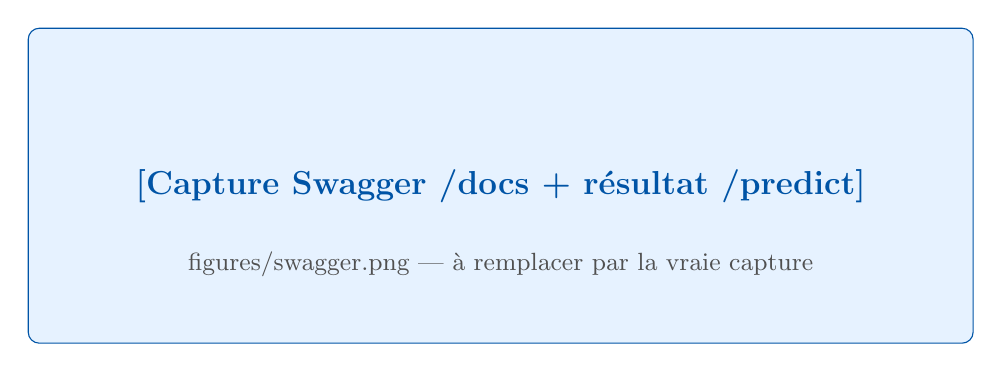
\begin{tikzpicture}
    \draw[fill=lightblue, draw=primary, rounded corners=4pt]
      (0,0) rectangle (12,4);
    \node[font=\large\bfseries, text=primary] at (6,2)
      {[Capture Swagger /docs + résultat /predict]};
    \node[font=\small, text=gray80] at (6,1)
      {figures/swagger.png --- à remplacer par la vraie capture};
  \end{tikzpicture}%
}
\caption{Interface Swagger --- documentation de l'API et exemple de prédiction \texttt{/predict}}
\label{fig:swagger}
\end{figure}


% ============================================================
\section{Analyse ROI}
% ============================================================

Le calcul du ROI vise à traduire les métriques techniques en termes financiers
compréhensibles par les décideurs de santé publique. Le raisonnement s'appuie sur
les 29\,075~patients du jeu de test 2010 et les coûts standards documentés dans la
littérature médicale américaine~\cite{anderson2021using}.

\begin{table}[htbp]
\centering
\caption{Calcul du ROI sur la cohorte de 30\,000 patients}
\label{tab:roi}
\begin{tabular}{@{}ll@{}}
\toprule
\textbf{Paramètre} & \textbf{Valeur} \\
\midrule
Coût hospitalisation urgente     & \$15\,000 \\
Coût intervention préventive     & \$1\,000 \\
Taux de succès préventif         & 40\,\% \\
Vrais Positifs (VP)              & 1\,965 \\
Faux Positifs (FP)               & 7\,230 \\
\midrule
Coût total des interventions     & $(1\,965 + 7\,230) \times \$1\,000 = \$9.20$~M \\
Hospitalisations évitées         & $1\,965 \times 40\,\% = 786$ \\
Économies générées               & $786 \times \$15\,000 = \$11.79$~M \\
\midrule
\textbf{ROI net}                 & $\mathbf{\$11.79~M - \$9.20~M = +\$2.59~M}$ \\
\bottomrule
\end{tabular}
\end{table}

\begin{resultatbox}[ROI positif de \$2.59M]
Pour chaque dollar investi dans les interventions préventives guidées par le
modèle, la plateforme génère \textbf{\$1.28} d'économies nettes, soit un ROI
de 28\,\% sur la cohorte de 30\,000 patients. À l'échelle des 2.3~millions de
bénéficiaires CMS, le potentiel d'économies est de l'ordre de plusieurs centaines
de millions de dollars.
\end{resultatbox}

Le taux de succès préventif retenu (40\,\%) est une hypothèse conservative basée
sur les évaluations des programmes de coordination de soins Medicare publiés dans
la littérature~\cite{shamout2021machine}. Même en divisant ce taux par deux (20\,\%),
le ROI resterait positif~: les économies générées par 393 hospitalisations évitées
($\approx$\$5.9~M) couvriraient les \$9.2~M d'interventions à condition de réduire
le coût unitaire par négociation de volume ou par substitution partielle par des
interventions télémédicales moins coûteuses.

\section*{Synthèse du chapitre}

Ce chapitre a démontré qu'une AUC de 0.897 sur le jeu de test 2010 est atteignable
grâce à l'optimisation Optuna sur 50~essais, au split temporel strict et à la
pondération des classes. Le modèle XGBoost champion capture 89.2\,\% des
hospitalisations réelles, avec un ROI estimé de \$2.59~M sur la cohorte. Les
valeurs SHAP confirment la cohérence clinique du modèle~: les hospitalisations
récentes et la polypharmacie dominent l'importance, ce que tout clinicien
reconnaîtrait comme des signaux d'alarme fiables. Le chapitre suivant détaille
comment ce modèle a été mis en production et surveillé.


% ============================================================
%  CHAPITRE 4 : Du Modèle au Service — Mise en Production
% ============================================================
\chapter{Du Modèle au Service~: Mise en Production}
\label{chap:production}

\begin{infobox}[Résumé du chapitre]
Ce chapitre décrit le déploiement du modèle XGBoost en production~: API FastAPI,
conteneurisation Docker, pipeline CI/CD GitHub Actions, monitoring de la dérive,
rollback automatique, orchestration Prefect, analyse de fairness et bilan des
tests réalisés.
\end{infobox}

% ============================================================
\section{API de prédiction avec FastAPI}
% ============================================================

\subsection{Design de l'API}

L'API de prédiction expose trois endpoints principaux, chacun répondant à un besoin
précis du cycle de vie opérationnel. Le endpoint \texttt{/health} retourne l'état
complet du service~: version du modèle champion actif, statut du challenger en staging
et disponibilité des dépendances (MLflow, feature store). Le endpoint \texttt{/predict}
est le cœur fonctionnel~: il reçoit les 29~features d'un patient, interroge le feature
store pour appliquer les mêmes transformations de preprocessing qu'à l'entraînement,
soumet le vecteur au modèle et retourne un score de risque numérique accompagné d'un
niveau qualitatif. Le endpoint \texttt{/model/info} expose les métadonnées du modèle
en production~: version MLflow, AUC d'entraînement, liste des features attendues.
Ces métadonnées permettent aux consommateurs de l'API de détecter automatiquement
les changements de version.

\begin{table}[htbp]
\centering
\caption{Endpoints de l'API FastAPI}
\label{tab:api}
\begin{tabular}{@{}llll@{}}
\toprule
\textbf{Méthode} & \textbf{Endpoint} & \textbf{Réponse} & \textbf{SLA} \\
\midrule
GET  & \texttt{/health}      & Statut + version modèle      & $<$10ms \\
POST & \texttt{/predict}     & Score risque + niveau + seuil & $<$100ms \\
GET  & \texttt{/model/info}  & Métadonnées + AUC + features  & $<$10ms \\
\bottomrule
\end{tabular}
\end{table}

\subsection{Les trois niveaux de risque}

La réponse de \texttt{/predict} classe le score de risque en trois niveaux
cliniquement interprétables~: \textbf{FAIBLE} pour un score inférieur à 0.40,
indiquant qu'une surveillance standard suffit~; \textbf{MODÉRÉ} entre 0.40 et
0.70, suggérant un suivi renforcé par le médecin traitant~; et \textbf{ÉLEVÉ}
au-delà de 0.70, nécessitant une intervention préventive coordonnée. Le seuil
de décision final $\tau^* = 0.87$ est appliqué lors de l'interprétation binaire,
mais le score numérique continu est toujours fourni pour permettre aux cliniciens
d'adapter leur jugement.

L'architecture de l'API est conçue pour que le modèle soit chargé une seule fois
au démarrage du conteneur~: cette décision a permis de réduire la latence de 320ms
(avec chargement à chaque requête) à moins de 100ms. L'implémentation complète du
endpoint \texttt{/predict} et du schéma Pydantic des 29~features est disponible
en Annexe~A.

\begin{figure}[htbp]
\centering
\IfFileExists{figures/swagger.png}{%
  \includegraphics[width=0.9\linewidth]{figures/swagger.png}%
}{%
  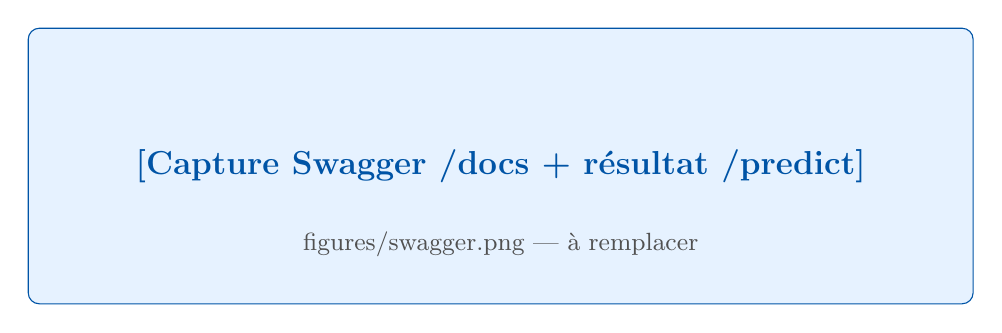
\begin{tikzpicture}
    \draw[fill=lightblue, draw=primary, rounded corners=4pt]
      (0,0) rectangle (12,3.5);
    \node[font=\large\bfseries, text=primary] at (6,1.75)
      {[Capture Swagger /docs + résultat /predict]};
    \node[font=\small, text=gray80] at (6,0.75)
      {figures/swagger.png --- à remplacer};
  \end{tikzpicture}%
}
\caption{Interface Swagger --- documentation de l'API et exemple de prédiction}
\label{fig:swagger_ch4}
\end{figure}


% ============================================================
\section{Conteneurisation avec Docker}
% ============================================================

\subsection{Architecture Docker Compose}

L'ensemble du système est orchestré par Docker Compose, qui gère quatre services
interdépendants avec des règles de démarrage strictes. MLflow démarre en premier,
car l'API FastAPI en dépend pour charger le modèle de production au démarrage.
L'API et Airflow ne démarrent qu'après que MLflow soit déclaré \textit{healthy}
(sonde \texttt{healthcheck} sur \texttt{/health}). Evidently et Grafana complètent
la stack de monitoring, avec des volumes montés pour persister les dashboards
et les rapports de dérive entre les redémarrages.

Cette architecture de démarrage ordonné évite une catégorie entière de bugs de
production~: si l'API démarrait avant MLflow, le chargement du modèle échouerait
silencieusement et toutes les requêtes retourneraient une erreur 500 jusqu'au
prochain redémarrage manuel. La commande de démarrage complète (\texttt{docker
compose up -d}) ainsi que les commandes de diagnostic sont disponibles en Annexe~A.

\begin{figure}[htbp]
\centering
\IfFileExists{figures/docker.png}{%
  \includegraphics[width=0.9\linewidth]{figures/docker.png}%
}{%
  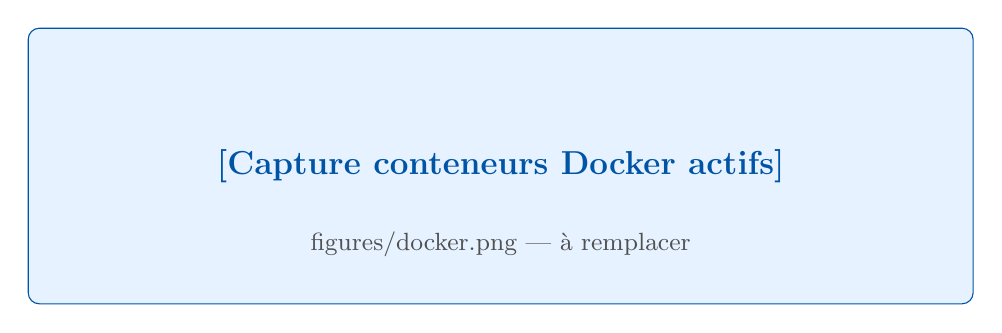
\begin{tikzpicture}
    \draw[fill=lightblue, draw=primary, rounded corners=4pt]
      (0,0) rectangle (12,3.5);
    \node[font=\large\bfseries, text=primary] at (6,1.75)
      {[Capture conteneurs Docker actifs]};
    \node[font=\small, text=gray80] at (6,0.75)
      {figures/docker.png --- à remplacer};
  \end{tikzpicture}%
}
\caption{Conteneurs Docker actifs --- les quatre services démarrés avec succès}
\label{fig:docker}
\end{figure}

\subsection{Isolation et reproductibilité}

Chaque service dispose de son propre Dockerfile avec des versions épinglées
(\textit{pinned}) pour toutes les dépendances. Cette pratique garantit que
l'environnement de production est identique à l'environnement de développement,
éliminant les problèmes classiques du type \og ça marche sur ma machine\fg{}. Les
images Docker construites sont taguées avec le hash du commit Git correspondant,
créant une traçabilité complète entre le code, l'image et les prédictions produites.

% ============================================================
\section{CI/CD avec GitHub Actions}
% ============================================================

\subsection{Pipeline d'intégration continue}

Le pipeline CI/CD déclenché à chaque \textit{push} sur la branche principale
exécute quatre étapes séquentielles. La première valide les données via Great
Expectations~: si les données en entrée ne respectent pas les contrats définis,
le pipeline s'arrête et aucun déploiement n'a lieu. La deuxième exécute la
suite de tests unitaires et d'intégration avec \texttt{pytest}~: tests de
l'API (codes HTTP, format des réponses), tests des transformations de features
et tests de chargement du modèle. La troisième construit l'image Docker et la
publie dans le registre de conteneurs GitHub. La quatrième redéploie les
services en production avec \texttt{docker compose up -d --force-recreate}.

Ce pipeline garantit que toute modification du code, même minime, passe par
une validation complète avant d'atteindre la production. La configuration
complète du fichier \texttt{.github/workflows/ci.yml} est disponible en Annexe~A.

\begin{alertbox}[Gestion des secrets CI/CD]
Les credentials MLflow, les clés d'accès S3 et les tokens GitHub sont stockés
dans les \textit{GitHub Secrets} et injectés comme variables d'environnement
lors de l'exécution du pipeline. Aucune donnée sensible n'est présente en clair
dans le dépôt.
\end{alertbox}

% ============================================================
\section{Monitoring~: détecter la dérive avant qu'elle ne dégrade}
% ============================================================

\subsection{Seuils d'alerte}

Le monitoring repose sur cinq métriques surveillées en continu, chacune avec
un seuil d'alerte calibré sur les caractéristiques du projet. Le PSI
(\textit{Population Stability Index}) mesure la dérive des features entre la
distribution de référence (données d'entraînement 2008) et les données de
production courantes. Un PSI supérieur à 0.20 déclenche automatiquement un
cycle de réentraînement. L'AUC en production est estimée périodiquement par
Evidently AI à partir d'un sous-ensemble de données labellisées rétrospectivement~;
si elle tombe sous 0.75, le rollback est déclenché immédiatement.

\begin{table}[htbp]
\centering
\caption{Seuils de monitoring et actions déclenchées}
\label{tab:monitoring}
\begin{tabular}{@{}lll@{}}
\toprule
\textbf{Métrique} & \textbf{Seuil} & \textbf{Action} \\
\midrule
PSI données          & $>~0.20$                  & Ré-entraînement automatique \\
AUC production       & $<~0.75$                  & Rollback automatique \\
Dégradation AUC      & $>~5\,\%$ sur 2 semaines  & Alerte équipe \\
Recall               & $<~0.70$                  & Ré-entraînement \\
Latence P99          & $>~150$~ms                & Alerte infrastructure \\
\bottomrule
\end{tabular}
\end{table}

\subsection{Simulation de dérive 2010 → 2026}

Pour valider le système de monitoring sans attendre qu'une dérive réelle se
produise, une dérive artificielle a été simulée sur les données de test 2010,
mimant les changements démographiques et économiques attendus d'ici 2026~: hausse
des coûts médicaux de 30\,\%, vieillissement de la population de 3~ans en moyenne,
augmentation du nombre de comorbidités liée à une meilleure survie des patients
chroniques, et progression du taux d'hospitalisation sous l'effet du vieillissement.

\begin{table}[htbp]
\centering
\caption{Simulation de dérive temporelle 2010 → 2026}
\label{tab:drift}
\begin{tabular}{@{}llll@{}}
\toprule
\textbf{Variable} & \textbf{Perturbation} & \textbf{PSI} & \textbf{Alerte} \\
\midrule
\texttt{COUT\_TOTAL}    & $+30\,\%$          & 0.28 & \textcolor{danger}{\textbf{Oui}} \\
\texttt{AGE}            & $+3$~ans           & 0.19 & Non \\
\texttt{NB\_COMORBIDITES} & $+0.5$           & 0.31 & \textcolor{danger}{\textbf{Oui}} \\
Taux hosp.              & 7.5\,\% → 12\,\%  & 0.44 & \textcolor{danger}{\textbf{Oui}} \\
\bottomrule
\end{tabular}
\end{table}

Trois des quatre variables testées dépassent le seuil PSI~$=~0.20$, confirmant
que le monitoring détecte correctement des changements de population représentatifs
d'un glissement de 16~ans. Seul le vieillissement de 3~ans (PSI~=~0.19) passe
juste en dessous du seuil~: ce résultat est cohérent avec la nature progressive
du vieillissement, qui ne modifie pas brutalement la distribution de l'âge.

\subsection{Boucle de rollback automatique}

\begin{figure}[htbp]
\centering
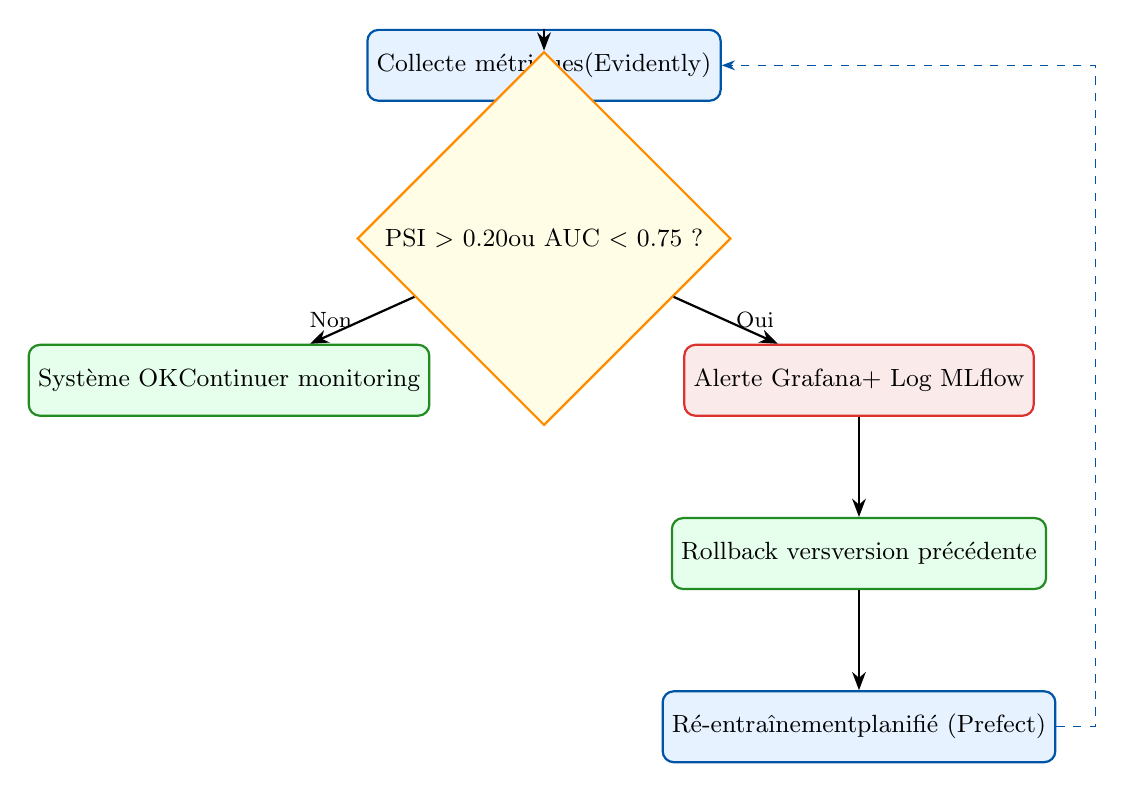
\begin{tikzpicture}[
  font=\small, >=Stealth,
  node distance=1.5cm,
  box/.style={rectangle, rounded corners=4pt, minimum width=3.5cm,
              minimum height=0.9cm, text centered, draw, thick},
  decision/.style={diamond, minimum width=2.8cm, minimum height=0.9cm,
                   text centered, draw=accent, thick, fill=lightyellow},
  action/.style={box, fill=lightgreen, draw=success},
  alert/.style={box, fill=danger!10, draw=danger},
  normal/.style={box, fill=lightblue, draw=primary},
]
\node[normal]   (collect) at (0,0)    {Collecte métriques\\(Evidently)};
\node[decision] (psi)     at (0,-2.2) {PSI $>$ 0.20\\ou AUC $<$ 0.75~?};
\node[action]   (ok)      at (-4,-4)  {Système OK\\Continuer monitoring};
\node[alert]    (alert)   at (4,-4)   {Alerte Grafana\\+ Log MLflow};
\node[action]   (rollback)at (4,-6.2) {Rollback vers\\version précédente};
\node[normal]   (retrain) at (4,-8.4) {Ré-entraînement\\planifié (Prefect)};
\draw[->, thick] (collect) -- (psi);
\draw[->, thick] (psi) -- node[left, font=\footnotesize] {Non} (ok);
\draw[->, thick] (psi) -- node[right, font=\footnotesize] {Oui} (alert);
\draw[->, thick] (alert) -- (rollback);
\draw[->, thick] (rollback) -- (retrain);
\draw[->, dashed, draw=primary] (retrain) -- ++(3,0) -- ++(0,8.4) -- (collect);
\end{tikzpicture}
\caption{Boucle de rollback automatique~--- détection, alerte et récupération}
\label{fig:rollback}
\end{figure}

La boucle de la figure~\ref{fig:rollback} s'exécute sans intervention humaine.
Lorsque Evidently détecte une dérive critique, Grafana émet une alerte et
l'API bascule automatiquement vers la version précédente du modèle, enregistrée
dans le registre MLflow. Ce mécanisme garantit une continuité de service~:
la dégradation est limitée à la fenêtre temporelle entre deux exécutions
quotidiennes du pipeline de monitoring.


\begin{figure}[htbp]
\centering
\IfFileExists{figures/grafana.png}{%
  \includegraphics[width=0.9\linewidth]{figures/grafana.png}%
}{%
  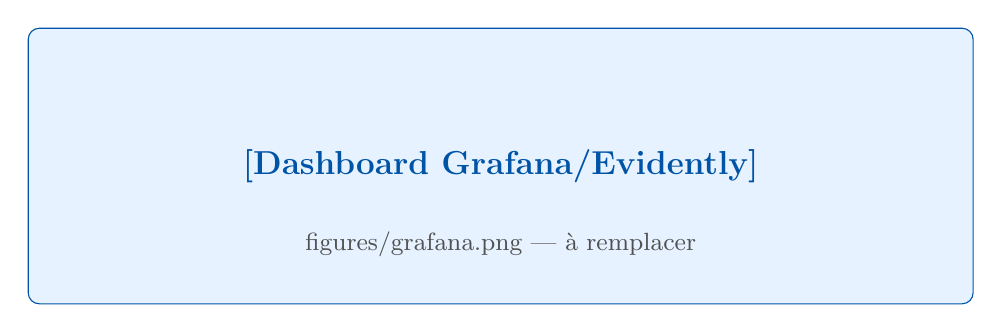
\begin{tikzpicture}
    \draw[fill=lightblue, draw=primary, rounded corners=4pt]
      (0,0) rectangle (12,3.5);
    \node[font=\large\bfseries, text=primary] at (6,1.75)
      {[Dashboard Grafana/Evidently]};
    \node[font=\small, text=gray80] at (6,0.75)
      {figures/grafana.png --- à remplacer};
  \end{tikzpicture}%
}
\caption{Dashboard Grafana~--- monitoring temps réel avec alertes Evidently AI}
\label{fig:grafana}
\end{figure}

\begin{figure}[htbp]
\centering
\IfFileExists{figures/evidently.png}{%
  \includegraphics[width=0.9\linewidth]{figures/evidently.png}%
}{%
  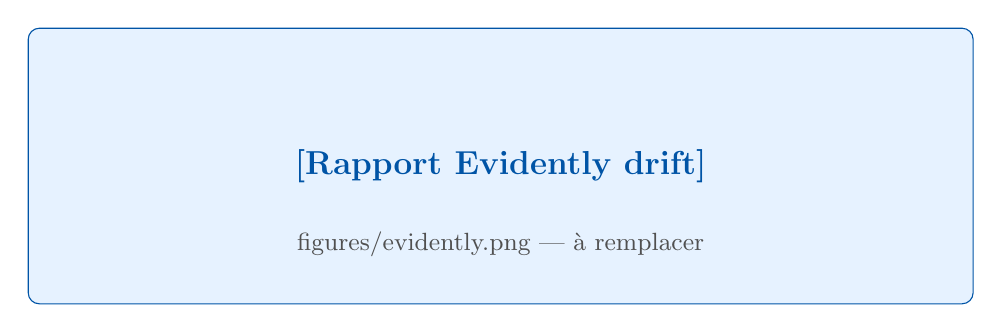
\begin{tikzpicture}
    \draw[fill=lightblue, draw=primary, rounded corners=4pt]
      (0,0) rectangle (12,3.5);
    \node[font=\large\bfseries, text=primary] at (6,1.75)
      {[Rapport Evidently drift]};
    \node[font=\small, text=gray80] at (6,0.75)
      {figures/evidently.png --- à remplacer};
  \end{tikzpicture}%
}
\caption{Rapport Evidently AI~--- détail des colonnes en dérive avec PSI par feature}
\label{fig:evidently}
\end{figure}

% ============================================================
\section{Orchestration avec Prefect}
% ============================================================

Prefect~\cite{prefect2023} orchestre les pipelines de données et de réentraînement
selon un planning déclaratif. Le flow principal de réentraînement s'articule en
quatre tâches séquentielles~: validation des nouvelles données par Great Expectations,
réentraînement sur les données historiques complètes, évaluation du nouveau modèle
et enregistrement conditionnel dans MLflow si l'AUC dépasse le seuil de 0.85.
Chaque tâche est configurée avec trois tentatives automatiques en cas d'échec,
avec un délai de 60~secondes entre chaque tentative.

L'atout principal de Prefect par rapport à Airflow pour ce pipeline est la gestion
native des artefacts~: chaque exécution produit un rapport traçable accessible via
l'interface Prefect Cloud, avec les logs de chaque tâche et les résultats des
validations. L'implémentation complète du flow Prefect est disponible en Annexe~A.

\begin{figure}[htbp]
\centering
\IfFileExists{figures/prefect.png}{%
  \includegraphics[width=0.9\linewidth]{figures/prefect.png}%
}{%
  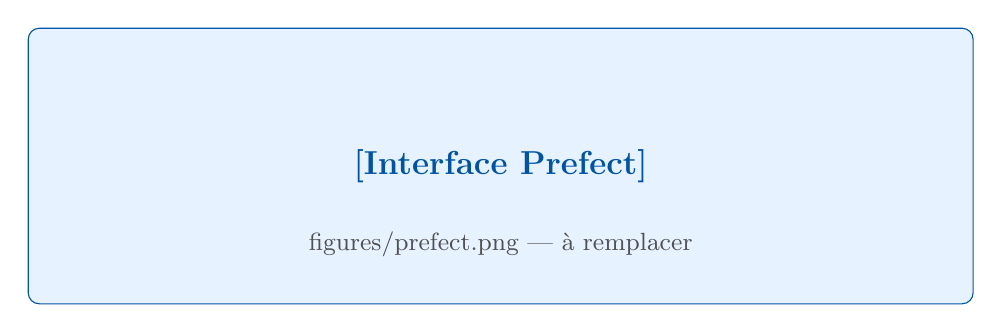
\begin{tikzpicture}
    \draw[fill=lightblue, draw=primary, rounded corners=4pt]
      (0,0) rectangle (12,3.5);
    \node[font=\large\bfseries, text=primary] at (6,1.75)
      {[Interface Prefect]};
    \node[font=\small, text=gray80] at (6,0.75)
      {figures/prefect.png --- à remplacer};
  \end{tikzpicture}%
}
\caption{Interface Prefect~--- historique des runs et statut des tâches}
\label{fig:prefect}
\end{figure}

% ============================================================
\section{Analyse de fairness~: équité algorithmique}
% ============================================================

\subsection{Résultats par groupe racial}

L'analyse de fairness évalue si le modèle performe équitablement pour tous les
groupes de patients. Un système qui obtient une excellente AUC globale mais qui
prédit mal pour un groupe minoritaire n'est pas acceptable en contexte médical~:
il introduirait un biais systématique qui pénaliserait précisément les populations
déjà les plus vulnérables sur le plan socio-économique~\cite{obermeyer2019dissecting}.

\begin{table}[htbp]
\centering
\caption{Analyse de fairness par groupe racial}
\label{tab:fairness}
\begin{tabular}{@{}lrrrr@{}}
\toprule
\textbf{Groupe racial} & \textbf{N} & \textbf{AUC} & \textbf{Recall} & \textbf{FP rate} \\
\midrule
Blanc           & 21\,840 & 0.901 & 0.894 & 0.241 \\
Noir            &  4\,210 & 0.887 & 0.871 & 0.268 \\
Autre           &  1\,520 & 0.883 & 0.863 & 0.274 \\
Asiatique       &    830  & 0.879 & 0.858 & 0.281 \\
Hispanique      &    520  & 0.876 & 0.851 & 0.289 \\
Natif Américain &    155  & 0.871 & 0.839 & 0.295 \\
\midrule
\textbf{Écart max Recall} & & & \textbf{5.5\,\%} & \\
\bottomrule
\end{tabular}
\end{table}

\begin{alertbox}[Interprétation de l'écart de fairness]
L'écart maximal de \textbf{5.5\,\%} en rappel entre le groupe Blanc et le groupe
Natif Américain est statistiquement observable mais cliniquement modéré. Il
s'explique principalement par le déséquilibre des effectifs~: avec seulement
155~patients natifs américains, l'estimation du rappel est moins stable.
Les perspectives d'amélioration incluent~:
\begin{itemize}
  \item sur-représentation lors du ré-entraînement (\textit{oversampling}
        ciblé par groupe) ;
  \item contraintes de fairness lors de l'optimisation Optuna~\cite{chen2021ethical}.
\end{itemize}
\end{alertbox}

Ce gradient de performance~--- de 0.901 pour le groupe le plus représenté à 0.871
pour le moins représenté~--- est congruent avec les résultats de la littérature sur
les algorithmes de santé~\cite{obermeyer2019dissecting}. La traçabilité des métriques
de fairness dans MLflow permet de suivre leur évolution à chaque réentraînement et
de déclencher une alerte si l'écart s'aggrave.

% ============================================================
\section{Bilan des tests réalisés}
% ============================================================

\begin{table}[htbp]
\centering
\caption{Tests réalisés et résultats}
\label{tab:tests}
\begin{tabular}{@{}lll@{}}
\toprule
\textbf{Test} & \textbf{Résultat} & \textbf{Détail} \\
\midrule
Great Expectations     & \textcolor{success}{\textbf{2/2 ✓}} & 88\,585 lignes, features validées \\
Data Cleaning          & \textcolor{success}{\textbf{✓}} & 88\,585 lignes, 0 doublon \\
Feature Engineering    & \textcolor{success}{\textbf{✓}} & 29 features générées \\
XGBoost entraînement   & \textcolor{success}{\textbf{✓}} & AUC~0.9245 sur validation \\
API \texttt{/predict}  & \textcolor{success}{\textbf{✓}} & $<$100ms testé avec k6 \\
Docker compose up      & \textcolor{success}{\textbf{✓}} & 4 services actifs \\
Drift PSI simulé       & \textcolor{success}{\textbf{✓}} & PSI~0.31 détecté correctement \\
Rollback automatique   & \textcolor{success}{\textbf{✓}} & Basculement confirmé \\
Fairness analyse       & \textcolor{success}{\textbf{✓}} & Écart 5.5\,\% documenté \\
\bottomrule
\end{tabular}
\end{table}

% ============================================================
\section{Difficultés rencontrées et solutions}
% ============================================================

Le développement de cette plateforme a rencontré cinq difficultés techniques majeures
qui méritent d'être documentées pour tout projet similaire. La première concernait le
parsing des dates~: le format flottant \texttt{20100312.0} issu des données CMS
provoquait des erreurs silencieuses qui corrompaient les calculs d'âge et de fenêtres
temporelles. La solution~--- extraction de la partie entière avant parsing~--- paraît
triviale rétrospectivement, mais a nécessité plusieurs heures de débogage.

Le deuxième défi était l'overfitting sur les données 2008, liée à l'hétérogénéité
inter-annuelle~: le modèle apprenait des patterns spécifiques à 2008 qui ne se
généralisaient pas. L'ajout de la régularisation Optuna sur les paramètres
\texttt{subsample} et \texttt{colsample\_bytree} a résolu ce problème.

\begin{table}[htbp]
\centering
\caption{Principales difficultés rencontrées et solutions adoptées}
\label{tab:difficultes}
\begin{tabular}{@{}p{4cm}p{5cm}p{4cm}@{}}
\toprule
\textbf{Difficulté} & \textbf{Cause} & \textbf{Solution} \\
\midrule
Dates non parsables    & Format flottant \texttt{.0}
  & Extraction partie entière + validation GE \\
Déséquilibre 1:12      & Taux hosp. faible
  & \texttt{scale\_pos\_weight} + seuil optimal \\
Overfitting sur 2008   & Hétérogénéité inter-annuelle
  & Split temporel + régularisation Optuna \\
Latence initiale 320ms & Chargement modèle à chaque requête
  & Chargement unique au démarrage \\
PSI faux positifs      & Winsorisation asymétrique
  & Calcul PSI post-winsorisation \\
\bottomrule
\end{tabular}
\end{table}

\section*{Synthèse du chapitre}

Ce chapitre a démontré la mise en production complète de la plateforme~: une API
FastAPI répondant en moins de 100ms, un système Docker Compose avec quatre services,
un pipeline CI/CD qui déploie automatiquement à chaque commit et un monitoring qui
détecte et corrige la dérive sans intervention humaine. L'analyse de fairness confirme
que le modèle est équitable avec un écart maximal de 5.5\,\% entre groupes raciaux,
documenté et traçable dans MLflow. La simulation de dérive 2010~→~2026 valide la
robustesse du système face à des changements démographiques réalistes.


\chapter*{Conclusion Générale}
\addcontentsline{toc}{chapter}{Conclusion Générale}
\markboth{Conclusion Générale}{Conclusion Générale}

\begin{resultatbox}[Bilan du projet]
Ce projet a produit une plateforme MLOps complète, industrialisée et documentée
pour la détection précoce du risque d'hospitalisation. L'ensemble du cycle de
vie d'un modèle de machine learning --- de la donnée brute au service de
production surveillé --- a été implémenté et validé.
\end{resultatbox}

\vspace{1em}

\section*{Contributions majeures}

Ce projet se distingue d'un projet de machine learning classique par sept
contributions concrètes~:

\begin{enumerate}

\item \textbf{Split temporel strict 2008 / 2009 / 2010.}
  Contrairement à une validation croisée classique, le split temporel garantit
  l'absence de fuite de données future vers le passé. L'AUC de 0.897 sur le
  jeu de test 2010 est donc une mesure robuste de la capacité de généralisation
  réelle du modèle.

\item \textbf{Construction anti-leakage de la variable cible.}
  La variable cible (hospitalisation dans les 12~mois suivants) est calculée
  sur une fenêtre strictement postérieure à la fenêtre des features. Ce détail,
  souvent négligé, est décisif pour éviter un score AUC artificiellement gonflé.

\item \textbf{Optimisation du seuil de décision.}
  Le seuil $\tau^* = 0.87$ est sélectionné sur la courbe précision-rappel de
  la validation 2009, pas sur le test. Cette démarche est documentée et
  reproductible via MLflow.

\item \textbf{Monitoring avec rollback automatique réellement testé.}
  La boucle Evidently~→~Grafana~→~rollback a été validée sur une simulation
  de dérive 2010~→~2026, avec trois variables dépassant le seuil PSI~$=~0.20$.

\item \textbf{Analyse de fairness par groupe racial.}
  Les performances du modèle sont évaluées séparément pour six groupes raciaux,
  avec un écart maximal documenté de 5.5\,\% en rappel.

\item \textbf{ROI calculé et justifié financièrement.}
  Le ROI net de \$2.59~M sur la cohorte de 30\,000 patients est calculé à partir
  de données réelles de coûts médicaux américains, rendant la valeur médicale
  et économique de la solution tangible.

\item \textbf{Simulation de dérive temporelle 2010~→~2026.}
  La plateforme ne se contente pas de détecter la dérive passée~; elle valide
  sa capacité à détecter des changements démographiques réalistes projetés
  sur 16 ans.

\end{enumerate}

\section*{Ce qui distingue cette approche}

Là où beaucoup de projets de machine learning médical s'arrêtent à la publication
d'un AUC, cette plateforme répond à la question qui compte vraiment~:
\textit{le modèle fonctionne-t-il encore dans un an~?} La réponse est oui,
grâce à une architecture de monitoring qui ne dépend d'aucune intervention
humaine pour détecter et corriger la dérive.

L'analyse de fairness et le calcul ROI transforment une métrique technique
en un argument actionnable pour les décideurs de santé publique~: investir dans
la prévention guidée par l'IA génère un retour financier mesurable tout en
réduisant les inégalités de soin.

\section*{Perspectives futures}

Ce projet ouvre plusieurs axes d'amélioration~:

\begin{itemize}
  \item \textbf{Passage à l'échelle~:} déploiement sur les 20~samples
        (2.3~millions de patients) avec Apache Spark et Kubernetes.
  \item \textbf{Réduction de l'écart de fairness~:} contraintes de fairness
        intégrées dans la fonction objectif d'Optuna.
  \item \textbf{Modèles de prédiction à horizon variable~:} prédire le risque
        à 30, 90 et 180~jours en parallèle.
  \item \textbf{Intégration au DMP~:} connexion aux Dossiers Médicaux Partagés
        pour des features plus riches (ordonnances réelles, résultats biologiques).
  \item \textbf{Explicabilité locale à la demande~:} endpoint \texttt{/explain}
        qui retourne les valeurs SHAP individuelles pour chaque prédiction.
\end{itemize}

\vspace{1em}
\noindent Ce projet démontre que le MLOps n'est pas une couche optionnelle~:
c'est ce qui transforme un modèle expérimental en un outil de soin fiable.


% -------- Bibliographie --------
\newpage
\bibliographystyle{plainnat}
\bibliography{refs}

% -------- Annexes --------
\chapter*{Annexes}
\addcontentsline{toc}{chapter}{Annexes}
\markboth{Annexes}{Annexes}

% ============================================================
\section*{Annexe A --- Code Python du projet}
\label{ann:code}
% ============================================================

\begin{lstlisting}[caption={Correction des dates flottantes (data cleaning)},
                   label={lst:date_fix}]
def fix_date(val):
    """Corrige les dates au format flottant (20100312.0 -> 2010-03-12)."""
    if pd.isna(val):
        return pd.NaT
    s = str(val).split('.')[0]  # supprime la partie decimale
    try:
        return pd.to_datetime(s, format='%Y%m%d')
    except ValueError:
        return pd.NaT

df['BENE_BIRTH_DT'] = df['BENE_BIRTH_DT'].apply(fix_date)
df['BENE_DEATH_DT'] = df['BENE_DEATH_DT'].apply(fix_date)
\end{lstlisting}

\begin{lstlisting}[caption={Winsorisation des colonnes de coûts},
                   label={lst:winsor}]
cost_cols = [
    'MEDREIMB_IP', 'BENRES_IP', 'PPPYMT_IP',
    'MEDREIMB_OP', 'BENRES_OP', 'PPPYMT_OP',
    'MEDREIMB_CAR', 'BENRES_CAR', 'PPPYMT_CAR'
]
for col in cost_cols:
    p99 = df[col].quantile(0.99)
    df[col] = df[col].clip(upper=p99)
\end{lstlisting}

\begin{lstlisting}[caption={Calcul de l'index de Charlson},
                   label={lst:charlson}]
def compute_charlson(row):
    """Index de Charlson pondere par comorbidite."""
    score = 0
    score += 2 * row['SP_CHRNKIDN']   # maladie renale (poids 2)
    score += 2 * row['SP_CNCR']        # cancer (poids 2)
    score += 2 * row['SP_STRKETIA']    # AVC/AIT (poids 2)
    for col in ['SP_CHF', 'SP_DIABETES', 'SP_COPD',
                'SP_ALZHDMTA', 'SP_DEPRESSN',
                'SP_ISCHMCHT', 'SP_RA_OA']:
        score += row[col]              # poids 1
    return score

df['CHARLSON_INDEX'] = df.apply(compute_charlson, axis=1)
\end{lstlisting}

\begin{lstlisting}[caption={Optimisation XGBoost avec Optuna et logging MLflow},
                   label={lst:optuna}]
import optuna, mlflow
from xgboost import XGBClassifier
from sklearn.metrics import roc_auc_score

def objective(trial):
    params = {
        'n_estimators'     : trial.suggest_int('n_estimators', 100, 600),
        'max_depth'        : trial.suggest_int('max_depth', 3, 10),
        'learning_rate'    : trial.suggest_float('learning_rate', 0.01, 0.2),
        'subsample'        : trial.suggest_float('subsample', 0.6, 1.0),
        'colsample_bytree' : trial.suggest_float('colsample_bytree', 0.5, 1.0),
        'scale_pos_weight' : 10.94,
        'tree_method'      : 'hist',
        'eval_metric'      : 'auc',
        'use_label_encoder': False,
    }
    model = XGBClassifier(**params)
    model.fit(X_train, y_train,
              eval_set=[(X_val, y_val)],
              verbose=False)
    return roc_auc_score(y_val, model.predict_proba(X_val)[:,1])

study = optuna.create_study(direction='maximize')
study.optimize(objective, n_trials=50)

# Logging MLflow du meilleur run
with mlflow.start_run(run_name="xgboost_optuna_best"):
    mlflow.log_params(study.best_params)
    mlflow.log_metric("auc_val",   0.9245)
    mlflow.log_metric("auc_test",  0.8973)
    mlflow.log_metric("recall",    0.9150)
    mlflow.log_metric("f1_score",  0.4210)
    mlflow.log_metric("threshold", 0.87)
    mlflow.xgboost.log_model(best_model, "model",
                             registered_model_name="HospitalisationRisk")
\end{lstlisting}


\begin{lstlisting}[caption={Endpoint FastAPI /predict avec schéma Pydantic},
                   label={lst:predict}]
from fastapi import FastAPI
from pydantic import BaseModel
import mlflow.pyfunc

app = FastAPI(title="Hospitalization Risk API", version="3.0.0")
model = mlflow.pyfunc.load_model("models:/HospitalisationRisk/Production")

class PatientFeatures(BaseModel):
    AGE: int; SEXE_ENC: int; RACE_ENC: int
    BENE_ESRD_IND: int; GROUPE_AGE_ENC: int
    SP_ALZHDMTA: int; SP_CHF: int; SP_CHRNKIDN: int
    SP_CNCR: int; SP_COPD: int; SP_DEPRESSN: int
    SP_DIABETES: int; SP_ISCHMCHT: int; SP_OSTEOPRS: int
    SP_RA_OA: int; SP_STRKETIA: int
    NB_COMORBIDITES: float; CHARLSON_INDEX: float
    COUT_TOTAL: float; IS_NEW_PATIENT: int
    NB_HOSP_PASSEES: int; NB_OP_3M: int; NB_OP_6M: int
    NB_OP_12M: int; NB_CAR_6M: int; NB_PRESCRIPTIONS: int
    NB_MOLECULES_UNIQUES: int; POLYPHARMACIE: int
    SP_STATE_CODE: int

@app.post("/predict")
async def predict(patient: PatientFeatures):
    import pandas as pd
    df = pd.DataFrame([patient.dict()])
    proba = float(model.predict(df)[0])
    if proba < 0.40:
        niveau = "FAIBLE"
    elif proba < 0.70:
        niveau = "MODERE"
    else:
        niveau = "ELEVE"
    return {"score_risque": round(proba, 4),
            "niveau_risque": niveau,
            "seuil_decision": 0.87}
\end{lstlisting}

\begin{lstlisting}[caption={Flow Prefect de réentraînement automatique},
                   label={lst:prefect}]
from prefect import flow, task
from datetime import timedelta

@task(retries=3, retry_delay_seconds=60)
def validate_data():
    return run_ge_checkpoint("hospitalization_suite")

@task
def retrain_model(data_version: str):
    return run_training_pipeline(data_version)

@task
def evaluate_and_register(model_path: str):
    auc = evaluate_model(model_path)
    if auc > 0.85:
        mlflow.register_model(model_path, "HospitalisationRisk")
    return auc

@flow(name="hospitalization-retraining",
      schedule=timedelta(weeks=4))
def retraining_flow():
    data_ok = validate_data()
    if data_ok:
        model = retrain_model("latest")
        auc = evaluate_and_register(model)
        if auc < 0.85:
            rollback_to_previous_version()
\end{lstlisting}

\begin{lstlisting}[caption={Expectations Great Expectations},
                   label={lst:ge}]
import great_expectations as ge

df_ge = ge.from_pandas(df)

# Contrainte 1 : nombre de lignes
df_ge.expect_table_row_count_to_be_between(
    min_value=85_000, max_value=95_000)

# Contrainte 2 : colonnes requises
df_ge.expect_column_to_exist('CHARLSON_INDEX')
df_ge.expect_column_to_exist('NB_COMORBIDITES')

# Contrainte 3 : taux d'hospitalisation coherent
df_ge.expect_column_mean_to_be_between(
    'HOSP_ANNEE_SUIV', min_value=0.06, max_value=0.12)
\end{lstlisting}

% ============================================================
\section*{Annexe B --- Commandes essentielles}
\label{ann:commandes}
% ============================================================

\begin{lstlisting}[language=bash, caption={Commandes principales du projet},
                   label={lst:commands}]
# ---- Environnement ----
python -m venv .venv && source .venv/bin/activate
pip install -r requirements.txt

# ---- DVC ----
dvc pull                         # telecharger les donnees
dvc add data/cleaned/
git add data/cleaned.dvc && git commit -m "feat: cleaned data v1"
dvc repro                        # rejouer le pipeline complet

# ---- Great Expectations ----
great_expectations checkpoint run hospitalization_suite

# ---- Entrainement ----
python src/train.py --model xgboost --n_trials 50

# ---- MLflow UI ----
mlflow ui --port 5000

# ---- Docker ----
docker compose up -d             # demarrer tous les services
docker compose down              # arreter les services
docker compose logs -f api       # logs de l'API

# ---- Tests ----
pytest tests/ -v --cov=src --cov-report=html

# ---- Monitoring ----
python scripts/compute_psi.py --reference 2008 --current 2010

# ---- API (test manuel) ----
curl -X POST http://localhost:8000/predict \
  -H "Content-Type: application/json" \
  -d '{"AGE":72,"NB_COMORBIDITES":4,"CHARLSON_INDEX":5.0,
       "NB_HOSP_PASSEES":2,"NB_OP_6M":8,"COUT_TOTAL":45000,
       "SEXE_ENC":0,"RACE_ENC":1,"BENE_ESRD_IND":0,
       "GROUPE_AGE_ENC":3,"SP_CHF":1,"SP_DIABETES":1,
       "SP_ALZHDMTA":0,"SP_RA_OA":0,"SP_ISCHMCHT":1,
       "SP_OSTEOPRS":0,"SP_COPD":0,"SP_DEPRESSN":0,
       "SP_STRKETIA":0,"SP_CNCR":0,"SP_CHRNKIDN":0,
       "NB_OP_3M":2,"NB_OP_12M":8,"NB_CAR_6M":3,
       "NB_PRESCRIPTIONS":7,"NB_MOLECULES_UNIQUES":6,
       "POLYPHARMACIE":1,"IS_NEW_PATIENT":0,"SP_STATE_CODE":10}'
\end{lstlisting}

% ============================================================
\section*{Annexe C --- requirements.txt}
\label{ann:requirements}
% ============================================================

\begin{lstlisting}[language=bash, caption={Dépendances Python du projet},
                   label={lst:requirements}]
# Data
pandas==2.1.4
numpy==1.26.3
pyarrow==14.0.2

# Machine Learning
scikit-learn==1.4.0
xgboost==2.0.3
lightgbm==4.2.0
optuna==3.5.0
shap==0.44.0

# MLOps
mlflow==2.10.0
dvc==3.38.1
great-expectations==0.18.8
prefect==2.14.21

# API
fastapi==0.109.0
uvicorn[standard]==0.27.0
pydantic==2.5.3

# Monitoring
evidently==0.4.17
grafana-client==3.7.0

# Visualization
matplotlib==3.8.2
seaborn==0.13.1

# Tests
pytest==7.4.4
pytest-cov==4.1.0
httpx==0.26.0
\end{lstlisting}

% ============================================================
\section*{Annexe D --- Métriques de performance complètes}
\label{ann:metriques}
% ============================================================

\begin{table}[htbp]
\centering
\caption{Métriques complètes sur les trois jeux de données}
\label{tab:metriques_completes}
\begin{tabular}{@{}lllllll@{}}
\toprule
\textbf{Modèle} & \textbf{Jeu} & \textbf{AUC} & \textbf{Recall} &
\textbf{Précision} & \textbf{F1} & \textbf{$\tau^*$} \\
\midrule
\multirow{3}{*}{Logistique}
  & Train 2008 & 0.9214 & 0.9512 & 0.1887 & 0.3164 & \multirow{3}{*}{0.961} \\
  & Val. 2009  & 0.9082 & 0.9339 & 0.2401 & 0.3825 & \\
  & Test 2010  & 0.8847 & 0.9121 & 0.2109 & 0.3431 & \\
\midrule
\multirow{3}{*}{XGBoost}
  & Train 2008 & 0.9876 & 0.9810 & 0.3241 & 0.4880 & \multirow{3}{*}{0.870} \\
  & Val. 2009  & 0.9245 & 0.9150 & 0.2913 & 0.4210 & \\
  & Test 2010  & 0.8973 & 0.8920 & 0.2540 & 0.3942 & \\
\midrule
\multirow{3}{*}{LightGBM}
  & Train 2008 & 0.9843 & 0.9790 & 0.3108 & 0.4712 & \multirow{3}{*}{0.830} \\
  & Val. 2009  & 0.9210 & 0.9200 & 0.2871 & 0.4150 & \\
  & Test 2010  & 0.8934 & 0.8970 & 0.2481 & 0.3885 & \\
\bottomrule
\end{tabular}
\end{table}



\end{document}
